\documentclass[10pt]{article}
\usepackage[preprint]{tmlr}
% If accepted, use: \usepackage[accepted]{tmlr}
% For a non-anonymous preprint, use: \usepackage[preprint]{tmlr}

\usepackage{amsmath,amssymb,amsthm,mathtools}
\usepackage{booktabs,graphicx,enumitem,microtype,placeins,array,multirow,float}
\usepackage{hyperref}
\hypersetup{hidelinks,pdftitle={Coupling Matters: Finite-Horizon Transport Analysis for Quantized Masked Diffusion Language Models},pdfauthor={Munsik Kim},pdfsubject={Preprint / technical report; not peer reviewed}}
\usepackage{url}
\usepackage{xcolor}

\theoremstyle{plain}
\newtheorem{theorem}{Theorem}[section]
\newtheorem{proposition}[theorem]{Proposition}
\newtheorem{lemma}[theorem]{Lemma}
\newtheorem{corollary}[theorem]{Corollary}
\theoremstyle{definition}
\newtheorem{definition}[theorem]{Definition}
\theoremstyle{remark}
\newtheorem{remark}[theorem]{Remark}

\newcommand{\Xs}{\mathcal{X}}
\newcommand{\Vs}{\mathcal{V}}
\newcommand{\Mtok}{\mathsf{M}}
\newcommand{\Ind}[1]{\mathbf{1}\{#1\}}
\newcommand{\Wd}{W_{d}}
\newcommand{\Ex}{\mathbb{E}}
\renewcommand{\Pr}{\mathbb{P}}
\newcommand{\Dcrn}{D_{\mathrm{CRN}}}
\newcommand{\Dcmc}{D_{\mathrm{CMC}}}
\newcommand{\Bfs}{B_{\mathrm{FS}}}
\newcommand{\TV}{\mathrm{TV}}
\newcommand{\eps}{\varepsilon}
\newcommand{\Psrc}{\mathcal{P}_{\mathrm{src}}}
\newcommand{\proofapp}{\par\noindent\emph{Complete proof in Appendix~\ref{app:proofs}.}\par}

\title{Coupling Matters: Finite-Horizon Transport Analysis for\\Quantized Masked Diffusion Language Models}

\author{\name Munsik Kim \\
\addr Independent Researcher, Republic of Korea}

\def\month{August}
\def\year{2026}
\def\openreview{}

\begin{document}
\maketitle

\begin{abstract}
Post-training quantization (PTQ) of masked diffusion language models is often assessed through local reconstruction error, but iterative masked generation can turn a small local change into a different token, commit set, and subsequent state. The standard trajectory-KL route from local perturbation to output stability can therefore become infinite after a single support mismatch. We develop a finite-horizon transport analysis in which the \emph{coupling}---the rule used to synchronize full-precision and quantized generation---is an explicit part of the measured upper bound. The central masked-diffusion result bounds terminal distortion after the first divergence by the residual masked mass, exposing a separation between split incidence and split consequence. For product transitions, coordinatewise maximal coupling is one-step optimal for weighted Hamming; for sample-then-select samplers, proposal couplings remain valid after model-dependent selection. Simultaneous concentration yields fixed-suite and declared prompt-population guarantees. Across MDLM and SMDM checkpoints, six bit widths, 16--64 generated positions, and official-sampler temperature sweeps, the same output marginals can produce sharply different paired costs under different couplings, while no coupling universally minimizes terminal damage. We also report two preregistered negative investigations: frozen additive token metrics do not resolve Hamming saturation, and survival--residual calibration does not beat uniform clipping on the primary W4 GSM8K endpoint. These results delimit what coupling-aware transport analysis supports---and what it does not.\footnote{Generative AI tools were used as assistive tools for hypothesis refinement, code and artifact drafting, literature discovery, and manuscript editing. All mathematical statements, proofs, references, numerical claims, code, and artifacts were checked by the authors against frozen source data, independent calculations, and explicit audits. The author takes responsibility for the complete report.}
\end{abstract}

\noindent\textbf{Version note.} Technical report v1.0.0. Preprint; not peer reviewed.

\section{Introduction}
\label{sec:intro}

Masked diffusion language models (dLLMs) generate text by repeatedly resolving masked coordinates rather than committing tokens strictly from left to right~\citep{austin2021d3pm,hoogeboom2021argmax,campbell2022continuous,lou2024sedd,sahoo2024mdlm,nie2025smdm,nie2025llada,ye2025dream}. This parallel, iterative structure creates a quantization problem that is qualitatively different from perturbing a single feed-forward prediction. A small weight error can change a candidate token, reorder the global confidence frontier, alter which positions are committed, and redirect all subsequent states. Recent dLLM PTQ methods accordingly calibrate by mask state, denoising time, or decision frontier~\citep{lin2025qdllm,xu2025dllmquant,zhang2026quantdllm,yan2026starquant,huang2026faircalib}. What remains less clear is what output-law statement is licensed by local perturbation measurements.

\begin{figure}[t]
\centering
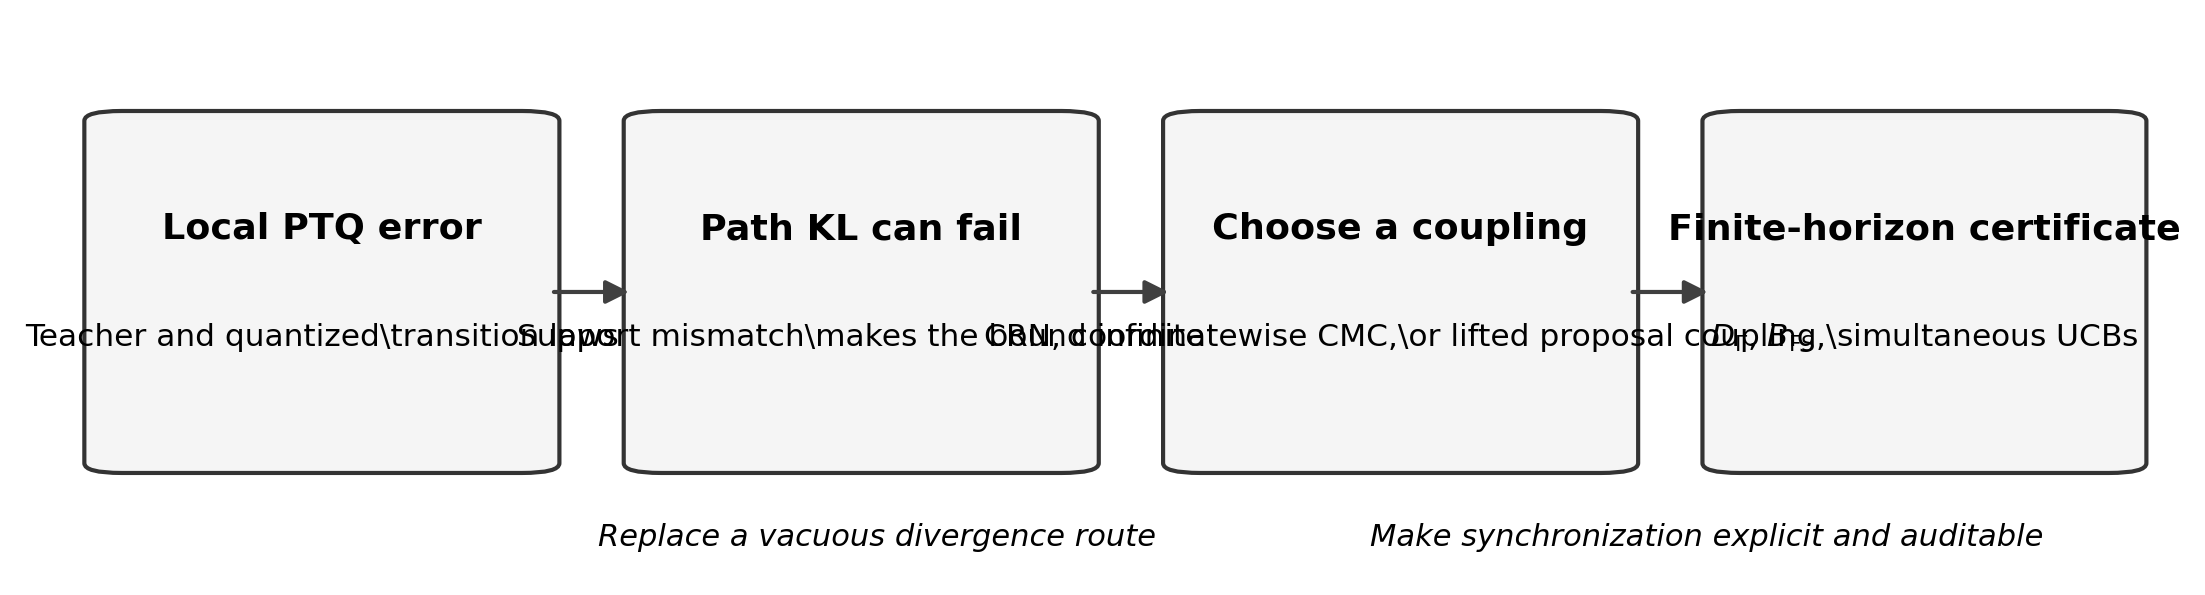
\includegraphics[width=.95\linewidth]{figures/figure_overview.png}
\caption{From local PTQ error to an output-law statement. A path-KL route can become infinite after support mismatch. Transport remains finite, but the result depends on the coupling used to synchronize the full-precision and quantized chains.}
\label{fig:overview}
\end{figure}

\paragraph{The obstruction.}
A conventional perturbation proof bounds KL divergence between full-precision (FP) and quantized trajectories and invokes data processing. For a masked decoder, however, a teacher-reachable transition may assign positive mass to a next state that the quantized transition assigns zero mass. The path KL is then infinite even when the terminal output laws are close. The divergence is a failure of the \emph{upper-bound route}, not evidence of catastrophic generation.

\paragraph{The coupling issue.}
We instead compare terminal laws with Wasserstein distance under normalized weighted Hamming. Any coupling $\Gamma$ of the two chains gives
\[
  \Wd(\mu_0^\star,\mu_0^q)
  \le D_\Gamma
  :=\Ex_\Gamma[d(X_0^\star,X_0^q)].
\]
The synchronization rule is therefore not a neutral implementation detail: it determines which valid upper bound is measured. This matters empirically. On the same W8 MDLM marginals, inverse-CDF common random numbers give terminal cost $0.9146$, whereas coordinatewise maximal coupling gives $0.2349$.

\paragraph{The masked-diffusion structure.}
The domain-specific idea is to stop at the first divergence. Under monotone copy-only generation, coordinates committed before the split cannot change again. Only the residual masked coordinates can contribute new terminal disagreement. This yields a diameter-safe bound whose two factors have distinct interpretations: bit width controls how often a split occurs, while the remaining reverse-time suffix controls how damaging that split can be.

\paragraph{Contributions.}
We make three claims.
\begin{enumerate}[leftmargin=1.6em,itemsep=2pt,topsep=2pt]
\item \textbf{Finite-horizon transport for irreversible masked generation.} We formalize the path-KL obstruction, derive teacher-prefix/quantized-suffix transport, and prove a first-divergence residual-mass bound together with finite-horizon and bounded-functional corollaries.
\item \textbf{Coupling-aware measurement.} For factorized transitions, coordinatewise maximal coupling exactly minimizes one-step weighted-Hamming cost. For non-factorized sample-then-select transitions, any proposal coupling can be pushed through the two deterministic, model-dependent selectors. We state explicitly what is one-step optimal and what is not.
\item \textbf{Statistical and empirical validation.} Simultaneous one-sided bounds cover both a fixed prompt suite and IID draws from a declared prompt population. Experiments isolate coupling, bit width, horizon, model, length, and sampler temperature. We also report preregistered negative investigations that fail to support stronger metric or calibration claims.
\end{enumerate}

\begin{table}[t]
\caption{Claims and evidence at a glance. Negative investigations narrow the interpretation rather than create additional contributions.}
\label{tab:claims}
\centering\small
\begin{tabular}{@{}p{.25\linewidth}p{.33\linewidth}p{.34\linewidth}@{}}
\toprule
Claim & Main evidence & Explicit boundary \\
\midrule
Path KL can be vacuous & support-mismatch proposition; deterministic selector examples & says nothing by itself about terminal task failure \\
First divergence controls worst-case damage & residual-mask theorem; early/middle/late damage $0.774/0.398/0.119$ & can be loose because splits may heal \\
Coupling changes the measured bound & W8 cost $0.915$ (CRN) vs. $0.235$ (CMC); official-sampler temperature panel & no universal coupling or path-optimality claim \\
Certificates extend beyond one suite & fixed-suite and prompt-population simultaneous UCBs; six-bit and second-model panels & exact-token metric; declared population only \\
Stronger metric/method claims are unsupported & additive-metric and calibration pilots & reported as negative investigations \\
\bottomrule
\end{tabular}
\end{table}

The intended contribution is therefore an analytical and measurement framework, not a new state-of-the-art quantizer. This positioning is deliberate: two follow-up attempts to turn the framework into a semantic metric and a transport-weighted calibration method did not pass their preregistered gates. Reporting those failures is part of the claim--evidence alignment of the paper.

\section{Related Work}
\label{sec:related}

\paragraph{Discrete diffusion and diffusion language models.}
Categorical diffusion has been developed through multinomial and structured discrete diffusion~\citep{hoogeboom2021argmax,austin2021d3pm}, continuous-time Markov-chain formulations~\citep{campbell2022continuous}, and ratio or score-entropy estimation~\citep{lou2024sedd}. Masked language variants scale denoising generation and flexible generation orders~\citep{sahoo2024mdlm,arriola2025bd3lm,nie2025smdm,nie2025llada,ye2025dream}. Work on early-decision bias and sampler correctness emphasizes that reverse-time selection is itself an experimental variable~\citep{kim2026early,tang2026sampler}. Our focus is not sampler quality relative to a data distribution, but perturbation between an FP sampler and a quantized sampler.

\paragraph{Diffusion convergence and error analysis.}
For continuous diffusion, convergence analyses relate score-estimation and discretization errors to sampling error~\citep{chen2023sampling,benton2024dlinear}. Discrete counterparts derive total-variation or KL guarantees for uniformization and $\tau$-leaping schemes~\citep{chen2024uniformization,ren2024discretecontinuous,liang2025absorb}. These works ask whether an approximate reverse process approaches a target distribution. We ask a different perturbation question: given two implemented masked samplers---FP and quantized---how can their finite-horizon output laws be compared when their supports and decision policies diverge?

\paragraph{LLM and dLLM quantization.}
Classical LLM PTQ includes second-order weight-only quantization~\citep{frantar2023gptq}, activation-aware scaling~\citep{lin2024awq}, activation smoothing~\citep{xiao2023smoothquant}, and rotation-based outlier removal~\citep{ashkboos2024quarot}. Recent dLLM work identifies activation outliers, state-dependent disparity, temporal accumulation, and fragile write frontiers~\citep{lin2025qdllm,xu2025dllmquant,zhang2026quantdllm,yan2026starquant,huang2026faircalib}. These methods primarily ask how to produce a better quantizer. Our primary question is orthogonal: for a fixed FP/quantized pair, what output-law statement is licensed, and how does the declared coupling affect that statement? A calibration pilot in Appendix~\ref{app:negative} tests whether the transport decomposition itself yields a better clipping rule; it does not beat uniform clipping on the primary task endpoint.

\paragraph{Coupling, transport, and Markov perturbation.}
Coupling and maximal-coupling constructions are standard tools for comparing stochastic processes~\citep{lindvall1992coupling}. Wasserstein perturbation bounds propagate local kernel differences through Markov dynamics~\citep{villani2009optimal,ollivier2009ricci,rudolf2018perturbation}. Our adaptation uses the irreversible copy-only structure of masked generation: after the first split, terminal damage is bounded by residual masked mass. Product structure gives an exact one-step additive-cost optimum, while proposal lifting handles model-dependent selection without claiming output-level maximality or terminal/path optimality.

\paragraph{Statistical certification and negative investigations.}
The statistical layer uses bounded concentration~\citep{hoeffding1963probability} to license simultaneous, prefix-closed horizon selection. The contribution is not the concentration inequality itself, but the explicit separation of fixed-suite and prompt-population estimands and the source-to-claim audit around them. We also report preregistered alternate-metric, lower-bound, and calibration investigations as negative evidence rather than selecting only successful follow-ups.

\section{Finite-Horizon Transport Framework}
\label{sec:framework}

\subsection{Setup}
Let $\Vs$ be a finite vocabulary, $\Mtok\notin\Vs$ a mask token, and $\Xs=(\Vs\cup\{\Mtok\})^N$. Reverse time runs $t=T,\ldots,0$. The FP and quantized kernels are $P_t,Q_t$, with a common initial law at $T$ and terminal laws $\mu_0^\star,\mu_0^q$. We use normalized weighted Hamming
\begin{equation}
 d(s,s')=\sum_{i=1}^N\lambda_i\Ind{s[i]\ne s'[i]},
 \qquad \lambda_i>0,\quad \sum_i\lambda_i=1,
 \label{eq:metric}
\end{equation}
so $\operatorname{diam}(d)=1$. A transition is \emph{monotone copy-only} if an already unmasked token is copied forever. For any coupling $\Gamma$ of the two chains,
\[
  \Wd(\mu_0^\star,\mu_0^q)
  \le D_\Gamma:=\Ex_\Gamma[d(X_0^\star,X_0^q)].
\]
For sample-then-select samplers, model $M\in\{\star,q\}$ first draws a proposal $\xi^M\sim\nu_t^M(\cdot\mid s)$ and then applies a deterministic, model-dependent map $\Phi_t^M(s,\xi^M)$. Thus $P_t=(\Phi_t^\star)_\#\nu_t^\star$ and $Q_t=(\Phi_t^q)_\#\nu_t^q$ at a common state.

\begin{table}[t]
\caption{The certificate map. Proofs and supporting statements are collected in Appendices~\ref{app:supporting}--\ref{app:proofs}.}
\label{tab:theory-map}
\centering\small
\begin{tabular}{@{}p{.22\linewidth}p{.28\linewidth}p{.41\linewidth}@{}}
\toprule
Result & Key assumption & What it licenses \\
\midrule
Path-KL obstruction & teacher-reachable support mismatch & the trajectory-KL upper-bound route can be infinite \\
Hybrid transport & finite state, common initial law & local kernel replacements propagated through a common suffix \\
First divergence & monotone copy-only & $D_\Gamma$ bounded by residual masked mass \\
Survival--hazard identity & synchronous coupling & split incidence and residual consequence separated by time \\
Coordinatewise optimum & product transition, additive cost & exact one-step Wasserstein cost \\
Lifted coupling & valid proposal coupling, deterministic selectors & a valid sample-then-select transition coupling \\
Concentration & bounded preregistered prompt blocks & simultaneous fixed-suite or prompt-population UCBs \\
\bottomrule
\end{tabular}
\end{table}

\subsection{Why trajectory KL can be vacuous}
Let $\mathbb P^\star,\mathbb P^q$ be trajectory laws on $\Xs^{T+1}$.
\begin{proposition}[Path-KL obstruction]
\label{prop:kl}
If some teacher-reachable state $s$ at step $t$ satisfies $P_t(s,\cdot)\not\ll Q_t(s,\cdot)$, then
$\mathrm{KL}(\mathbb P^\star\|\mathbb P^q)=\infty$. This includes deterministic transitions with different next states and deterministic commit-set selectors with different commit sets.
\end{proposition}
\proofapp
Data processing then supplies only an infinite upper bound on terminal KL. The terminal laws may still be close, so a finite metric route is needed.

\subsection{Hybrid transport}
Let $Q_{t-1:1}=Q_{t-1}\cdots Q_1$ and define the terminal effect of replacing one kernel at state $s$ by
\[
\eta_t(s)=\Wd\!\left(P_t(s,\cdot)Q_{t-1:1},Q_t(s,\cdot)Q_{t-1:1}\right).
\]
\begin{theorem}[Teacher-prefix/quantized-suffix transport]
\label{thm:hybrid}
With a common initial law,
\begin{equation}
\Wd(\mu_0^\star,\mu_0^q)
\le \sum_{t=1}^T\Ex_{S_t\sim\mu_t^\star}[\eta_t(S_t)].
\label{eq:hybrid}
\end{equation}
The teacher prefix determines occupancy and the quantized suffix determines propagation. Reversing the hybrid order yields the mirror pairing.
\end{theorem}
\proofapp
The raw telescoping sum can exceed the metric diameter because repeated kernel swaps charge the same terminal coordinate multiple times. The coordinate-union hierarchy in Appendix~\ref{app:supporting} charges each coordinate once. The sharper domain-specific statement stops at the first split.

\subsection{First divergence and residual masked mass}
Let $\tau$ be the first transition at which two coupled chains differ, and define residual masked mass
\[
R(s)=\sum_{i:s_i=\Mtok}\lambda_i.
\]
\begin{theorem}[First-divergence residual-mass bound]
\label{thm:fs}
For any coupling $\Gamma$ of monotone copy-only chains from a common initial state,
\begin{equation}
\Wd(\mu_0^\star,\mu_0^q)
\le D_\Gamma
\le \Bfs^\Gamma
:=\Ex_\Gamma[R(X_\tau)\Ind{\tau\ne\dagger}]
\le \Pr_\Gamma(\tau\ne\dagger)
\le1.
\label{eq:fs-main}
\end{equation}
The same statement holds at every deterministic finite horizon.
\end{theorem}
\proofapp
The argument uses the irreversible structure directly: before the first split both chains share the same committed tokens, and those coordinates remain fixed. Only coordinates still masked at the split can contribute new terminal cost.

For a synchronous coupling, let $G_t$ be survival without an earlier split and let $h_t^\Gamma(s)$ be the one-step split probability at a common state.
\begin{proposition}[Survival--hazard decomposition]
\label{prop:hazard}
Under the synchronous representation,
\begin{equation}
\Bfs^\Gamma
=\sum_{t=1}^T
\Ex\!\left[
\Ind{G_t}\,h_t^\Gamma(X_t)\,R(X_t)
\right].
\label{eq:hazard}
\end{equation}
\end{proposition}
\proofapp
Equation~\eqref{eq:hazard} separates three factors: survival to the current step, the probability of splitting now, and the maximal remaining consequence. It motivates the empirical analysis in Section~\ref{sec:mechanism}, but does not by itself imply that a local reconstruction loss is a valid surrogate for $h_t$.

For any fixed $f:\Xs\to[0,1]$, the split event also controls a bounded downstream functional.
\begin{corollary}[Bounded-functional stability]
\label{cor:functional}
At every deterministic horizon $r$,
\[
|\Ex f(X_r^\star)-\Ex f(X_r^q)|
\le \Pr_\Gamma(\tau^{(r)}\ne\dagger).
\]
\end{corollary}
\proofapp
This is a validity statement, not a claim that first-split probability tightly controls semantics or task accuracy.

\subsection{Coupling is part of the measurement}
Assume first that the actual one-step transitions factorize as $P_t=\bigotimes_i p_{t,i}^\star$ and $Q_t=\bigotimes_i p_{t,i}^q$. Let $\delta_{t,i}=\TV(p_{t,i}^\star,p_{t,i}^q)$.
\begin{theorem}[Coordinatewise maximal coupling]
\label{thm:cmc}
Independently maximally coupling each coordinate defines a valid transition coupling with split hazard
$h_t^{\mathrm{CMC}}=1-\prod_i(1-\delta_{t,i})$. Iteration yields a path coupling satisfying
$\Wd\le\Dcmc\le\Bfs^{\mathrm{CMC}}\le1$.
\end{theorem}
\proofapp
\begin{proposition}[One-step weighted-Hamming optimality]
\label{prop:cmc-onestep-opt}
For weighted Hamming,
\begin{equation}
\Wd(P_t(s,\cdot),Q_t(s,\cdot))
=\sum_i\lambda_i\delta_{t,i}(s),
\label{eq:cmc-opt}
\end{equation}
and coordinatewise maximal coupling attains the minimum.
\end{proposition}
\proofapp
This is additive one-step optimality. It is not joint maximality for the event $X\ne Y$ and does not imply terminal or path optimality.

For a sample-then-select transition, proposals are coupled before selection.
\begin{proposition}[Lifted proposal coupling]
\label{prop:lifted}
If $\pi_t$ couples $\nu_t^\star$ and $\nu_t^q$, then
$\Gamma_t^{\mathrm{lift}}=\operatorname{Law}(\Phi_t^\star(s,\xi^\star),\Phi_t^q(s,\xi^q))$
is a valid coupling of the actual transitions. Moreover,
\begin{align}
 h_t^{\mathrm{lift}}(s)\le&\ \Pr_{\pi_t}(\xi^\star\ne\xi^q)\\
 &+\Pr_{\pi_t}(\xi^\star=\xi^q,\ \Phi_t^\star(s,\xi^\star)\ne\Phi_t^q(s,\xi^q)).
 \label{eq:lift-channels}
\end{align}
\end{proposition}
\proofapp
The two terms are proposal/token and policy-selection channels. They are an upper-bound decomposition rather than an exact causal partition because different proposals can map to the same next state.
\begin{corollary}[Temperature-zero limit]
\label{cor:det-limit}
If both proposal laws are Dirac masses, the proposal coupling is unique. Coupling-choice comparisons disappear; splits are determined by proposal-token or deterministic policy-boundary differences.
\end{corollary}
\proofapp

\subsection{Simultaneous statistical statements}
For a fixed suite of $m$ prompts, $r_j$ independent coupling draws per prompt, and $K$ preregistered one-sided cells:
\begin{theorem}[Fixed-suite simultaneous concentration]
\label{thm:fixedsuite}
With probability at least $1-\delta$, simultaneously for all upper cells $j$,
\[
\mu_j\le\widehat\mu_j+
\sqrt{\frac{\log(K/\delta)}{2mr_j}}.
\]
\end{theorem}
\proofapp
For IID prompt draws $C_1,\ldots,C_m\sim\Psrc$, repeated coupling draws are first averaged within each prompt block.
\begin{theorem}[Prompt-population simultaneous concentration]
\label{thm:population}
With probability at least $1-\delta$, simultaneously for all upper cells,
\[
\nu_j\le\widehat\nu_j+
\sqrt{\frac{\log(K/\delta)}{2m}}.
\]
\end{theorem}
\proofapp
The estimands are distinct. The first controls the fixed-suite average over declared coupling randomness; the second controls expectation under the declared source population. Because every horizon cell is included in the simultaneous family, prefix-closed horizon selection is licensed without post-selection correction.

\section{Empirical Evidence}
\label{sec:experiments}

\subsection{Design and audit contract}
We use simulated matrix-weight, per-output-channel symmetric round-to-nearest (RTN), with activations left in the reference precision. The primary metric is normalized exact-token Hamming over generated positions. Each work package freezes the model and checkpoint, prompt source and IDs, bit grid, coupling draws, horizons, statistical family, and event-addressed random-number keys before outcomes are inspected. Table~\ref{tab:design} separates the estimands and purposes of the panels; Appendix~\ref{app:experiments} gives the complete protocols.

\begin{table}[t]
\caption{Experimental map. ``Population'' denotes IID draws from a frozen filtered WikiText-103 source-record population.}
\label{tab:design}
\centering\footnotesize
\setlength{\tabcolsep}{2pt}
\begin{tabular}{@{}p{.18\linewidth}p{.11\linewidth}p{.16\linewidth}p{.17\linewidth}p{.23\linewidth}@{}}
\toprule
Panel & Model & Prompt/length & Coupling & Purpose \\
\midrule
Fixed certificate & MDLM 0.2B & 64 fixed / 16 & CMC, CRN & coupling and horizon \\
Prompt population & MDLM 0.2B & 128 IID / 16 & CMC & source-population UCB \\
Finite-bit scaling & MDLM 0.2B & 64 IID / 16 & CMC & W3--W8 mechanism \\
Second model & SMDM 1.14B & 32 fixed / 16,64 & CMC, CRN & model/length transfer \\
Official selector & SMDM 1.14B & 32 fixed / 16 & lifted CMC, CRN & sample-then-select coupling \\
\bottomrule
\end{tabular}
\end{table}

Across the five primary pathwise families and the temperature extension, $29{,}664$ recorded trajectory--horizon checks satisfy their preregistered inequalities with zero violation. These are dependent audit checks, not independent statistical observations. Raw rows, per-trajectory checkpoints, source hashes, and independent reaggregation scripts are retained in the accompanying artifacts.

\subsection{The same marginals yield different coupling costs}
\label{sec:coupling-results}
Table~\ref{tab:fixed-pop} and Figure~\ref{fig:main-results} summarize the primary result. Under inverse-CDF common random numbers (CRN), W8 terminal cost is $0.9146$, close to the matched 16-token independent-FP distance $0.9766$. Coordinatewise maximal coupling (CMC) reduces the cost to $0.2349$ and keeps $48.4\%$ of trajectories synchronized through the full horizon. A separate 32-token intrinsic-diversity audit gives $0.9878$; it is not the matched reference for this panel.

\begin{table}[t]
\caption{Direct CMC mean and simultaneous one-sided 95\% UCB at full horizon. Fixed suite: $m=64,r=4,K=49$; prompt population: $m=128,K=49$.}
\label{tab:fixed-pop}
\centering\small
\begin{tabular}{@{}crrrr@{}}
\toprule
& \multicolumn{2}{c}{Fixed 64-prompt suite} & \multicolumn{2}{c}{Prompt population}\\
\cmidrule(lr){2-3}\cmidrule(l){4-5}
Bit & Mean & UCB & Mean & UCB\\
\midrule
W8 & 0.2349 & 0.3508 & 0.2832 & 0.4472\\
W6 & 0.4043 & 0.5203 & 0.4385 & 0.6025\\
W4 & 0.7671 & 0.8831 & 0.7996 & 0.9636\\
\bottomrule
\end{tabular}
\end{table}

\begin{figure}[t]
\centering
\begin{minipage}[t]{0.49\linewidth}
\centering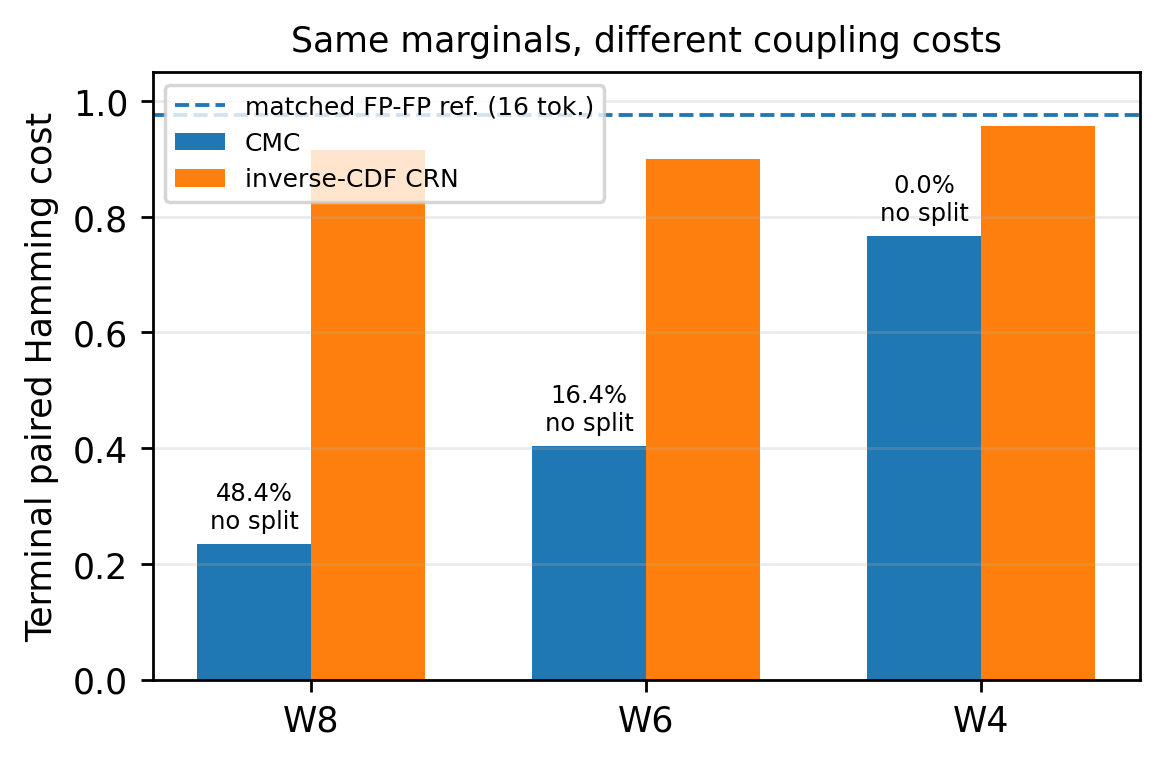
\includegraphics[width=\linewidth]{figures/figure_main_coupling.png}
\end{minipage}\hfill
\begin{minipage}[t]{0.49\linewidth}
\centering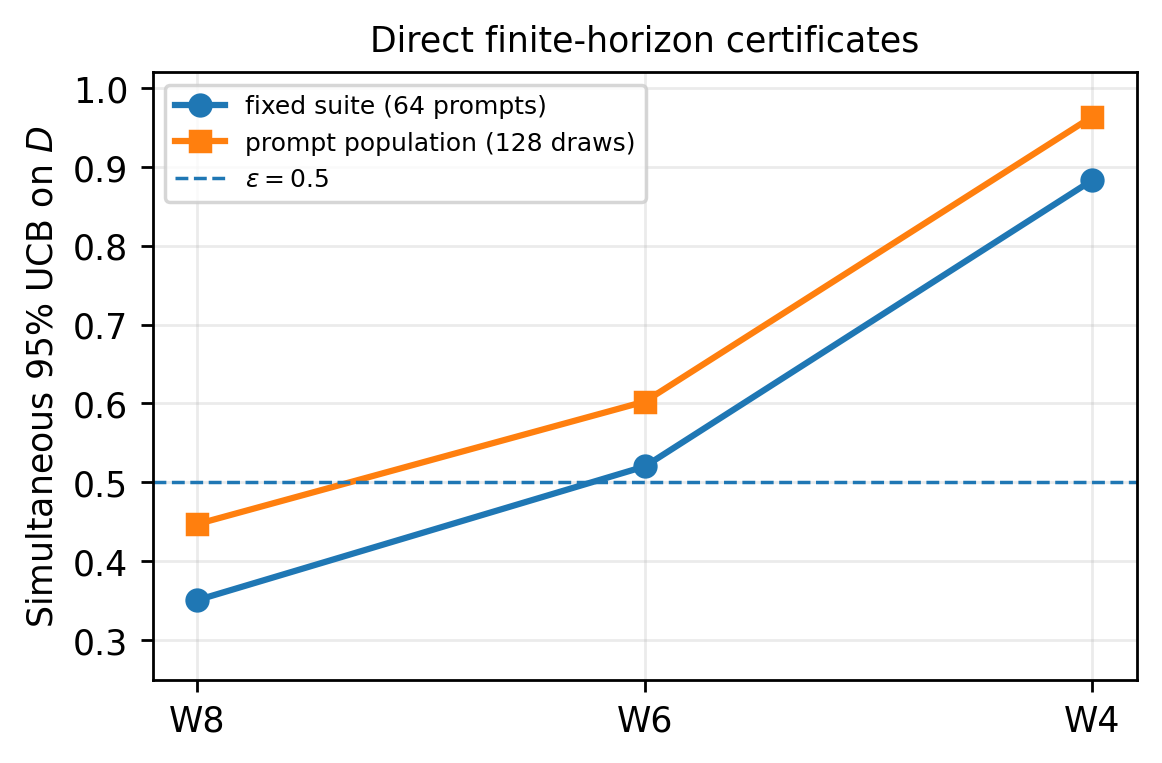
\includegraphics[width=\linewidth]{figures/figure_main_certificates.png}
\end{minipage}
\caption{\textbf{Left:} changing only the coupling changes the measured terminal cost. \textbf{Right:} direct simultaneous UCBs on the fixed suite and declared prompt population. A UCB above $0.5$ means that tolerance $0.5$ is not certified at full horizon; it is not a validity failure.}
\label{fig:main-results}
\end{figure}

The population panel preserves the aggregate precision ordering, but its estimand differs. At W8, trajectory-draw split probability changes from $0.5156$ on the fixed suite to $0.5781$ under the source-population experiment; trajectory-conditional endpoint damage changes from $0.455$ to $0.490$. Prompt-block any-split fractions ($0.805/0.969/1.000$) are reported separately and are not trajectory split probabilities.

\paragraph{Sensitivity to the within-prompt independence premise.}
The fixed-suite primary radius treats the four event-addressed coupling streams per prompt as independent bounded draws, as preregistered. A conservative prompt-block analysis first averages those draws and uses only $m=64$ blocks, doubling the radius from $0.11598$ to $0.23197$. The corresponding W8/W6/W4 direct UCBs are $0.4668/0.6363/0.9991$: W8 remains below $0.5$, whereas W6 and W4 weaken. We report both analyses because the primary statement relies on the standard idealization that independently addressed pseudorandom streams implement independent Monte Carlo draws.

\subsection{Incidence and consequence of the first split}
\label{sec:mechanism}
The first-divergence decomposition predicts two distinct quantities: how often a split occurs and how much unresolved suffix remains when it occurs. The data support that separation. Lower precision increases common-state mismatch incidence, while the same split is much more consequential early in reverse time than late (Figure~\ref{fig:mechanism}).

\begin{figure}[t]
\centering
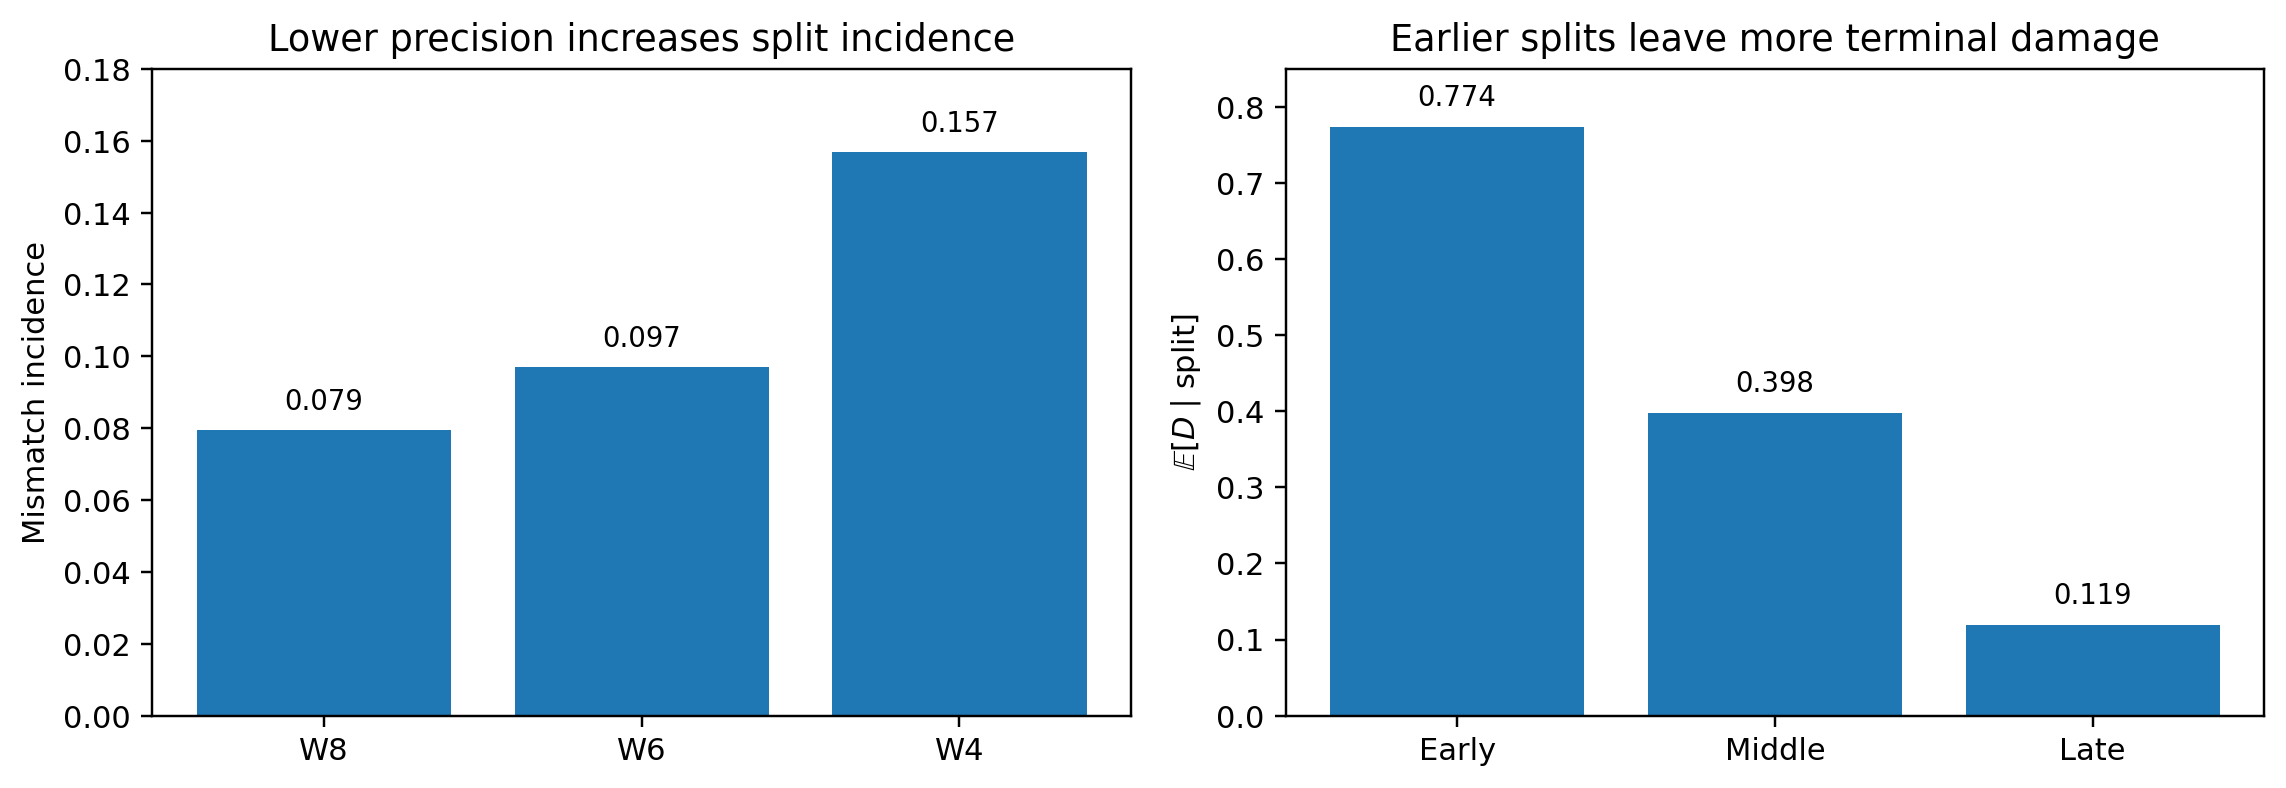
\includegraphics[width=.92\linewidth]{figures/figure_mechanism.png}
\caption{Mechanism behind terminal damage. \textbf{Left:} lower precision raises same-state mismatch incidence. \textbf{Right:} conditional terminal damage after an early split is far larger than after a late split.}
\label{fig:mechanism}
\end{figure}

The W8/W6/W4 mismatch incidences are $0.079/0.097/0.157$. Conditional terminal damage is $0.774$ for early, $0.398$ for middle, and $0.119$ for late splits. These values give empirical content to Equation~\eqref{eq:hazard}: bit width primarily changes the split hazard, while remaining masked mass and suffix length control the consequence. The identity is descriptive rather than an optimization theorem; Appendix~\ref{app:negative} reports a preregistered calibration attempt that failed to turn this decomposition into a task-improving method.

\subsection{Finite-bit scaling, model transfer, and task relevance}
A preregistered 32/32 calibration/held-out study evaluates W3--W8 on fresh prompt draws. Over the prespecified W4--W8 fit range, held-out prompt-fixed-effect slopes are
\[
\beta_W=0.7855\ [0.7618,0.8078],\qquad
\beta_H=0.7580\ [0.7346,0.7804],
\]
for exact one-step Wasserstein cost and CMC split hazard; within-prompt $R^2$ exceeds $0.96$. W3 is a preregistered stress point and is excluded from the primary fit. These are finite-range empirical summaries, not asymptotic quantization laws.

On a separate 1.14B SMDM checkpoint, direct CMC costs increase with lower precision at both 16 and 64 generated positions. Full-horizon direct UCBs at length 16 are $0.433/0.677/0.947$, and at length 64 are $0.599/0.807/0.993$ for W8/W6/W4. A separate 100-example GSM8K panel gives BF16/W8/W6/W4 accuracies $51/51/50/49\%$ with exact McNemar $p$-values $1.000/1.000/0.625$. It is deliberately described as task relevance evidence rather than a coupling certificate because that archived task run did not record a valid proposal coupling. The contrast between large exact-token CRN cost and unchanged W8 accuracy is one reason we do not interpret Hamming as a semantic or task-performance metric.

\subsection{Official sample-then-select sampler}
The SMDM task sampler first samples position-wise candidate tokens and then applies a global fixed-count confidence top-$k$ decision. We couple proposals and push them through the unchanged FP and quantized selectors. At temperature zero the proposal law is deterministic and coupling choice disappears, as predicted by Corollary~\ref{cor:det-limit}. At temperature $0.2$ the pushed-forward law is nearly deterministic. Raising temperature creates measurable support after selection: at temperature $1.0$, maximum empirical effective support is $1.449$ and minimum modal probability is $0.817$.

\begin{figure}[t]
\centering
\begin{minipage}[t]{0.64\linewidth}
\centering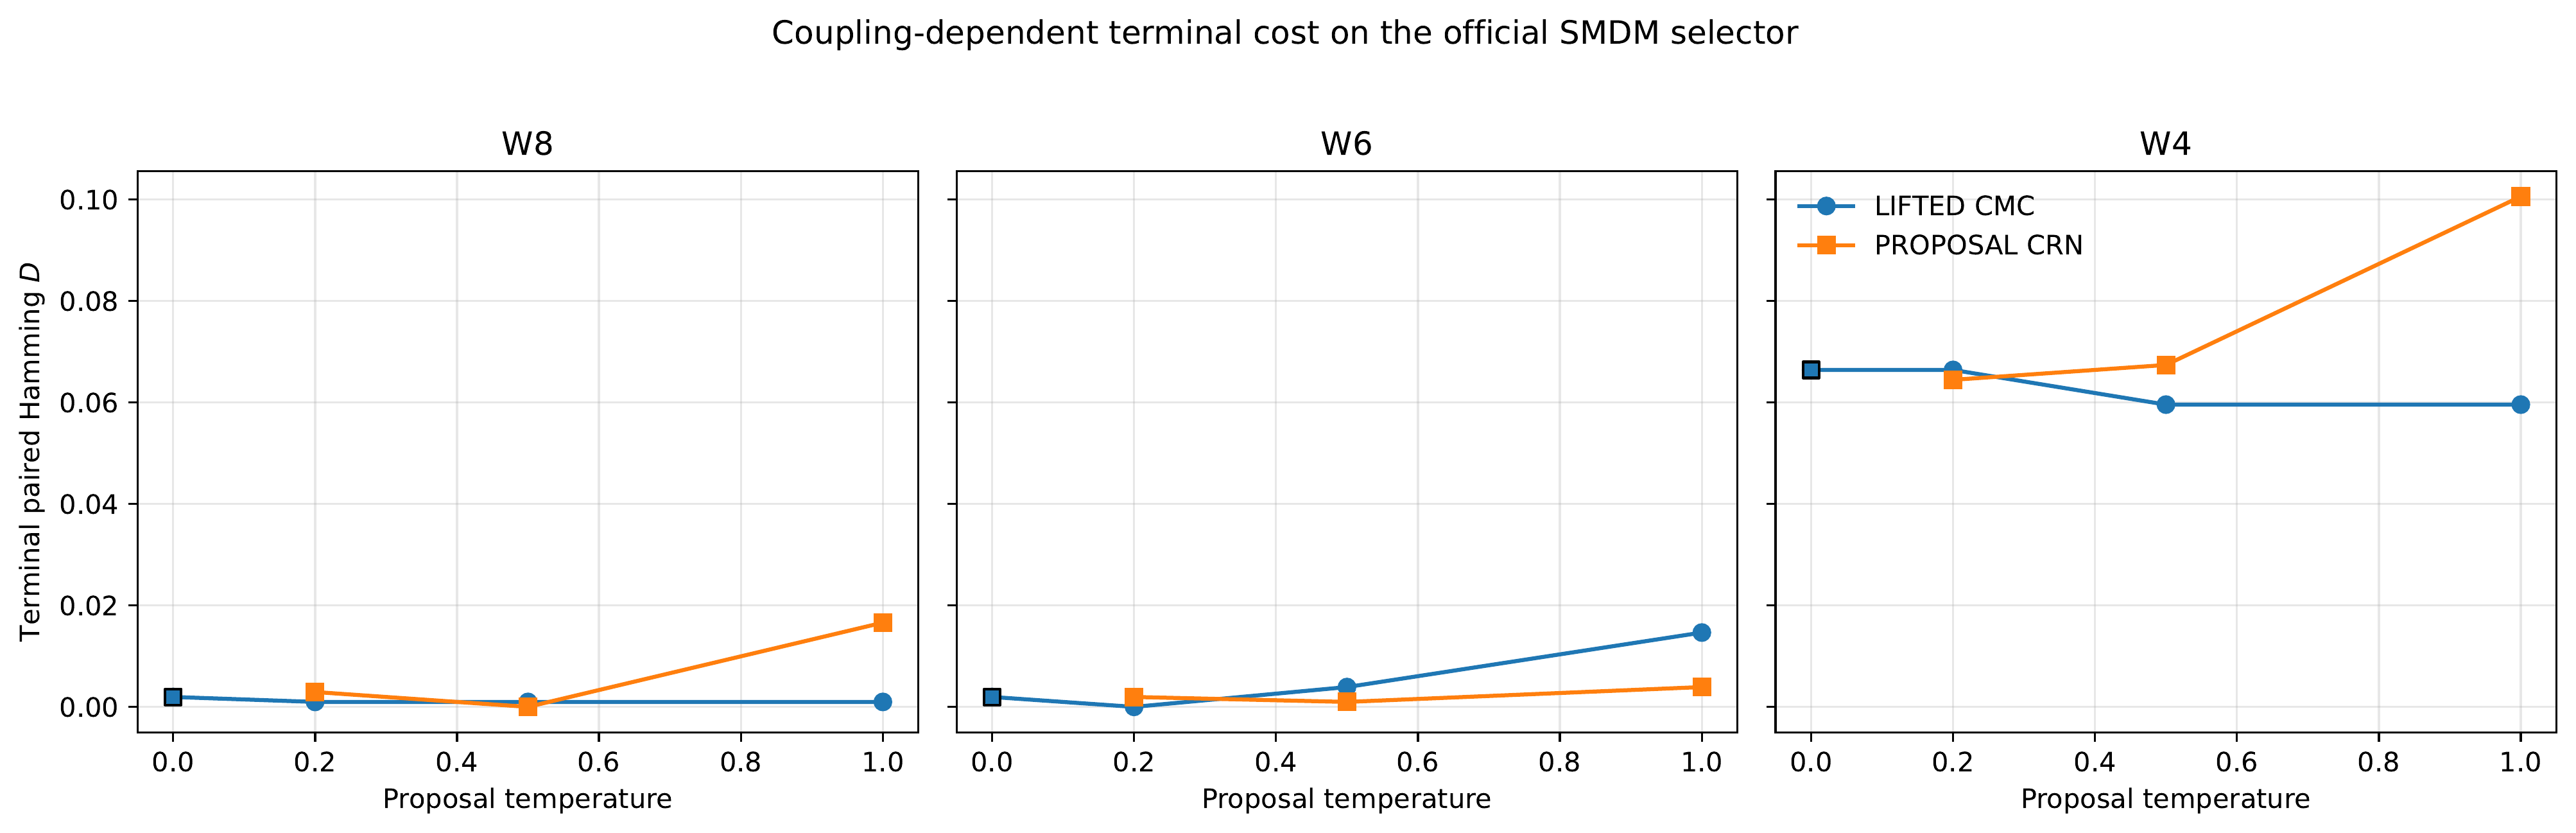
\includegraphics[width=\linewidth]{figures/figure_temperature_coupling_cost.png}
\end{minipage}\hfill
\begin{minipage}[t]{0.34\linewidth}
\centering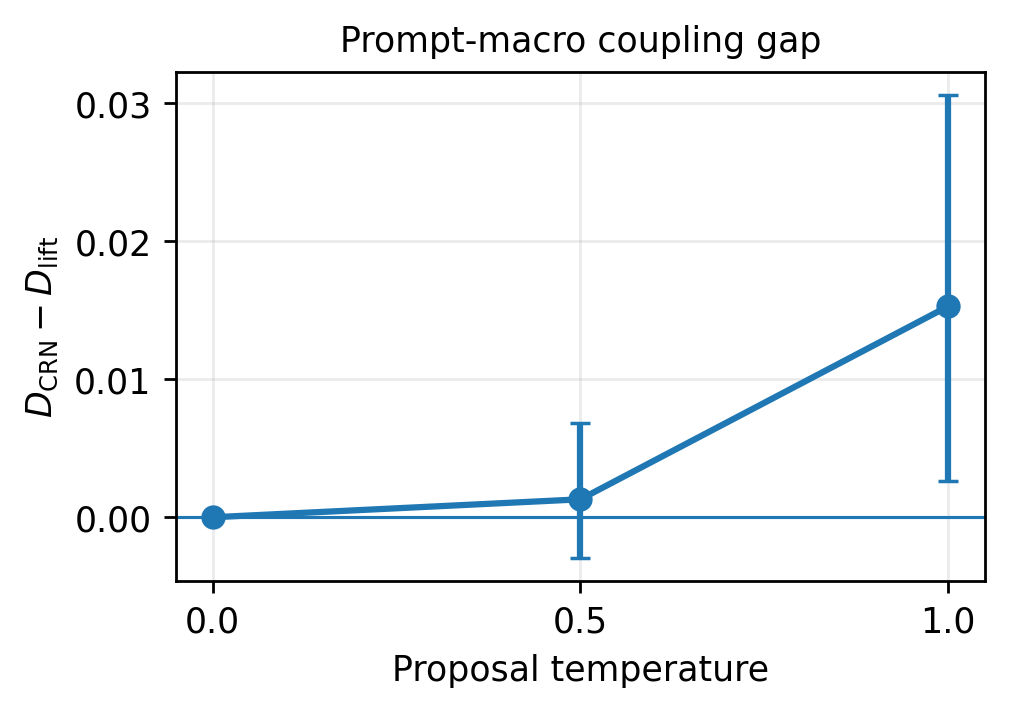
\includegraphics[width=\linewidth]{figures/figure_temperature_gap_compact.png}
\end{minipage}
\caption{Coupling dependence on the official sampler. \textbf{Left:} terminal cost by bit and proposal temperature. \textbf{Right:} prompt-macro $D_{\rm CRN}-D_{\rm lift}$ with paired prompt-cluster bootstrap intervals. The mean gap is positive at temperature $1.0$, but bit-level directions are mixed.}
\label{fig:temperature}
\end{figure}

At temperature $1.0$, the prompt-macro CRN-minus-lifted gap is $0.0153$ with bootstrap interval $[0.0026,0.0306]$, but the median gap is zero, the one-sided sign-test $p$-value is $0.166$ (Holm-adjusted $0.332$), and W6 reverses direction. Lifted CMC reduces proposal-vector mismatch from $0.1709$ to $0.0724$, yet post-selection next-state mismatch remains nearly unchanged ($0.0142$ versus $0.0146$): the selector maps many different proposals to the same next state. Conditional healing is also mixed across bits. Thus coupling dependence survives outside the deterministic limit, while proposal-level maximality does not induce a universal terminal-cost ordering.

\subsection{What the certificates do not establish}
All preregistered relative-to-reference-diversity certificates fail. First-divergence bounds can be loose because they intentionally ignore post-split healing. Exact-token Hamming is auditable and aligned with the theory, but it is not a semantic-quality certificate. The next section reports two preregistered investigations designed to test stronger interpretations; both return negative results.

\section{Preregistered Negative Investigations}
\label{sec:negative}

Two follow-up work packages tested whether the analysis could support materially stronger claims. Their designs, gates, and outcomes were fixed before evaluation. Neither investigation supports an additional positive contribution; we include them because they delimit the framework's interpretation and prevent post-hoc escalation of claims.

\subsection{Alternative additive metrics and terminal localization}
The first investigation generalized the product-transition result from $0$--$1$ token cost to any bounded additive token metric. For $d_c(x,y)=\sum_i\lambda_i c_i(x_i,y_i)$ and product laws $P=\bigotimes_i p_i$, $Q=\bigotimes_i q_i$, the exact identity
\[
W_{d_c}(P,Q)=\sum_i\lambda_i W_{c_i}(p_i,q_i)
\]
holds; Appendix~\ref{app:negative} gives the proof and a general-cost first-divergence corollary. The empirical question was whether a frozen token-embedding hybrid or tokenizer-byte metric would reduce the saturation seen under exact-token Hamming.

It did not. For W8 under CRN, the ratio of FP--quantized distance to independent-FP distance is $0.9365$ for Hamming, $0.9209$ for the embedding hybrid, and $0.9159$ for the byte hybrid. The alternative metrics mainly rescale disagreements and preserve nearly the same example ordering. On the 100-example GSM8K panel, answer-disagreement AUCs are $0.9845/0.9856/0.9876$ for Hamming/embedding/byte, while correctness-disagreement AUC is highest for Hamming ($0.9573$). We therefore retain exact Hamming as the theorem-aligned audit metric and do not present the alternatives as semantic metrics.

The same work package trained coordinatewise Kantorovich witnesses on the fixed suite and evaluated them on disjoint prompt-population draws. Point estimates at W4 were positive, but every simultaneous distribution-free lower confidence bound was zero. Hence the attempted terminal localization remains
$0\le W_d\le\mathrm{UCB}$ rather than a nontrivial lower/upper interval. The result does not imply that the true distance is small; it shows that the frozen prompt-independent witness and available sample size do not certify a positive lower bound.

\subsection{Survival--residual calibration pilot}
The second investigation asked whether the survival--residual decomposition could improve per-row clipping calibration. Calibration states were weighted by survival and residual masked mass, with uniform, margin-frontier, residual-only, and hazard-only baselines. The primary endpoint was held-out W4 GSM8K accuracy on 512 examples.

\begin{table}[H]
\caption{Primary W4 calibration result. Transport weighting improves some FP-fidelity metrics but not held-out task accuracy.}
\label{tab:negative-calibration}
\centering\small
\begin{tabular}{@{}lrrr@{}}
\toprule
Method & Accuracy & BF16 answer agreement & Terminal Hamming \\
\midrule
RTN absmax & 56.84\% & 84.57\% & 0.0534 \\
Uniform clipping & \textbf{57.42\%} & 87.50\% & 0.0472 \\
Margin frontier & 56.84\% & 88.48\% & 0.0405 \\
Transport SR & 56.64\% & \textbf{89.26\%} & \textbf{0.0381} \\
Transport SRH & 56.45\% & 88.67\% & 0.0364 \\
\bottomrule
\end{tabular}
\end{table}

Transport SR differs from RTN by $-0.20$ percentage points (95\% paired-bootstrap interval $[-1.95,1.37]$) and from uniform clipping by $-0.78$ points ($[-1.95,0.39]$). It reduces terminal Hamming relative to RTN and raises BF16 answer agreement, but does not improve ground-truth accuracy. The proposed surrogate bridge is also weak: state-level reconstruction perturbation predicts the next split with ROC AUC $0.545$ (95\% interval $[0.479,0.602]$), and its Spearman correlation with residual terminal damage is $0.052$. At W3, calibrated clipping broadly improves over absmax RTN, but transport weighting is not uniquely superior to uniform calibration.

These outcomes sharpen the scope of the paper. First-divergence analysis is useful for explanation and auditing, but the tested local reconstruction objective is not a reliable proxy for split risk. Similarly, closeness to the BF16 output need not improve task accuracy. We therefore make no algorithmic, semantic, or lower-bound localization claim from these follow-ups.

\section{Discussion, Reporting Guidance, and Limitations}
\label{sec:discussion}

\subsection{What is established}
The analysis supports three conclusions. First, path KL may be an unusable upper-bound route for masked generation because one policy or token decision can create support mismatch. Second, a finite transport statement requires a declared coupling: two couplings of the same marginal chains can yield substantially different paired costs. Third, monotone copy-only structure gives a domain-specific first-divergence bound in which split incidence and residual consequence are separated. The fixed-suite and prompt-population experiments, finite-bit study, second-model panel, and official-sampler temperature sweep support these conclusions under their declared estimands.

The direct and first-divergence routes serve different purposes. Direct paired cost is typically tighter but depends on the selected coupling. The residual-mass route is diameter-safe and mechanistically legible, but can be loose because it discards all post-split healing. A large gap between the two is therefore not a contradiction; it is evidence that transient policy-boundary differences often disappear before the terminal state.

\subsection{A minimal reporting standard}
A stability number for quantized masked generation is incomplete unless it identifies the experiment that defines it. We recommend reporting at least:
\begin{enumerate}[leftmargin=1.6em,itemsep=2pt,topsep=2pt]
\item the terminal metric and generated-position weights;
\item the coupling, including vocabulary order and post-split continuation;
\item the horizon and whether the result is direct or first-divergence based;
\item the statistical unit, simultaneous family, and confidence level;
\item the prompt estimand (fixed suite or a declared source population);
\item an intrinsic FP--FP reference and a task-relevance panel when available.
\end{enumerate}
For sample-then-select systems, proposal coupling and selector implementation should be audited separately. Event-addressed random streams are important: a preliminary stateful-RNG implementation produced 809 spurious pathwise violations that disappeared after semantic event addressing and replay tests.

\subsection{What is not established}
The title deliberately uses ``analysis'' rather than suggesting input-wise certified robustness. Our high-probability statements concern expected bounded costs over a fixed suite or declared prompt population. They are not deterministic per-input radii. Exact-token Hamming is a finite, auditable metric aligned with the product-coupling theory, but not a semantic or task metric. All relative-to-reference-diversity certificates fail. The bounded-functional corollary is formally valid, yet current first-split UCBs are too loose for a useful task-accuracy guarantee.

We also lack a nontrivial population lower confidence bound for terminal Wasserstein distance. The held-out coordinate-witness investigation in Section~\ref{sec:negative} yields zero formal LCBs, so the primary numerical results remain coupling-based upper bounds. The attempted additive token metrics do not resolve saturation, and the attempted transport-weighted calibration does not improve the primary W4 task endpoint. These failures are part of the evidence, not omitted alternatives.

\subsection{External validity}
Quantization is simulated matrix-weight RTN with reference-precision activations, not a deployment-kernel benchmark. The largest checkpoint is 1.14B. The prompt-population guarantee concerns a frozen filtered WikiText-103 source population, not arbitrary prompts, and official-sampler comparisons use a fixed 32-prompt suite. Large confidence/entropy samplers, activation quantization, hardware kernels, and substantially larger dLLMs remain external-validity questions. The present contribution is an analysis and measurement framework rather than a new state-of-the-art quantizer.

\section{Conclusion}
Local PTQ error does not by itself determine the stability of iterative masked generation. A finite statement requires a propagation argument, an explicit coupling, a horizon, and a statistical estimand. For monotone masked generation, first divergence and residual masked mass provide a simple domain-specific explanation of how local decisions can affect terminal outputs. Across the audited panels, coupling changes the measured upper bound, while no single coupling universally minimizes terminal damage. The negative investigations further show that neither a frozen token-level metric substitution nor a simple survival--residual calibration rule closes the gap to semantic or task-level guarantees. Quantized dLLM stability should therefore be reported as a carefully scoped transport analysis, together with the coupling and evidence that define it.


\section*{Broader impact}
This work studies the reliability of efficiency interventions for iterative language generation. Potential benefits include more transparent reporting of quantization-induced distribution shift and fewer misleading stability claims. The main risk is over-interpreting an exact-token transport bound as a semantic or task-performance guarantee. We mitigate that risk by separating fixed-suite and population estimands, reporting failed relative and task-level investigations, and explicitly limiting claims to the declared metrics, couplings, models, and samplers. The study uses public text corpora and benchmark data and does not involve human-subject data collection.

\section*{Reproducibility statement}
Appendix~\ref{app:proofs} contains complete proofs. The experimental appendices specify model and checkpoint identities, prompt populations, statistical families, coupling and event-addressed RNG contracts, negative investigations, and source-to-claim accounting. The supplementary source package contains anonymized manuscript code, figure data, compact audit ledgers, archive hashes, and model-free reproduction instructions; large public checkpoints and datasets are referenced by immutable identifiers rather than duplicated.

\clearpage
\small
\bibliographystyle{plainnat}
\begin{thebibliography}{99}

\bibitem[Arriola et~al.(2025)]{arriola2025bd3lm}
M.~Arriola, A.~Gokaslan, J.~Dao, A.~Gu, and V.~Smith.
Block diffusion: Interpolating between autoregressive and diffusion language models.
\emph{International Conference on Learning Representations}, 2025. Oral.

\bibitem[Ashkboos et~al.(2024)]{ashkboos2024quarot}
S.~Ashkboos, A.~Mohtashami, M.~L. Croci, B.~Fletcher, M.~Jaggi, D.~Alistarh, and T.~Hoefler.
QuaRot: Outlier-free 4-bit inference in rotated LLMs.
\emph{Advances in Neural Information Processing Systems}, 2024.

\bibitem[Austin et~al.(2021)]{austin2021d3pm}
J.~Austin, D.~D. Johnson, J.~Ho, D.~Tarlow, and R.~van~den Berg.
Structured denoising diffusion models in discrete state-spaces.
\emph{Advances in Neural Information Processing Systems}, 2021.

\bibitem[Benton et~al.(2024)]{benton2024dlinear}
J.~Benton, V.~De~Bortoli, A.~Doucet, and G.~Deligiannidis.
Nearly $d$-linear convergence bounds for diffusion models via stochastic localization.
\emph{International Conference on Learning Representations}, 2024. Spotlight.

\bibitem[Campbell et~al.(2022)]{campbell2022continuous}
A.~Campbell, J.~Benton, V.~De~Bortoli, T.~Rainforth, G.~Deligiannidis, and A.~Doucet.
A continuous time framework for discrete denoising models.
\emph{Advances in Neural Information Processing Systems}, 2022.

\bibitem[Chen et~al.(2023)]{chen2023sampling}
S.~Chen, S.~Chewi, J.~Li, Y.~Li, A.~Salim, and A.~R. Zhang.
Sampling is as easy as learning the score: Theory for diffusion models with minimal data assumptions.
\emph{International Conference on Learning Representations}, 2023. Notable top 5\%.

\bibitem[Chen and Ying(2024)]{chen2024uniformization}
H.~Chen and L.~Ying.
Convergence analysis of discrete diffusion model: Exact implementation through uniformization.
arXiv:2402.08095, 2024.

\bibitem[Cobbe et~al.(2021)]{cobbe2021gsm8k}
K.~Cobbe, V.~Kosaraju, M.~Bavarian, M.~Chen, H.~Jun, L.~Kaiser, M.~Plappert, J.~Tworek, J.~Hilton, R.~Nakano, C.~Hesse, and J.~Schulman.
Training verifiers to solve math word problems.
arXiv:2110.14168, 2021.

\bibitem[Frantar et~al.(2023)]{frantar2023gptq}
E.~Frantar, S.~Ashkboos, T.~Hoefler, and D.~Alistarh.
GPTQ: Accurate post-training quantization for generative pre-trained transformers.
\emph{International Conference on Learning Representations}, 2023.

\bibitem[Hoeffding(1963)]{hoeffding1963probability}
W.~Hoeffding.
Probability inequalities for sums of bounded random variables.
\emph{Journal of the American Statistical Association}, 58(301):13--30, 1963.

\bibitem[Hoogeboom et~al.(2021)]{hoogeboom2021argmax}
E.~Hoogeboom, D.~Nielsen, P.~Jaini, P.~Forr{\'e}, and M.~Welling.
Argmax flows and multinomial diffusion: Learning categorical distributions.
\emph{Advances in Neural Information Processing Systems}, 2021.

\bibitem[Huang et~al.(2026)]{huang2026faircalib}
H.~Huang et~al.
Frontier-aware instability-reweighted calibration for post-training quantization of diffusion large language models.
\emph{International Conference on Machine Learning}, 2026.

\bibitem[Kim et~al.(2026)]{kim2026early}
J.~Kim, S.~Choi, Y.~Jo, M.~Lee, and M.~Seo.
Early decisions matter: Proximity bias and initial trajectory shaping in non-autoregressive diffusion language models.
arXiv:2604.10567, 2026.

\bibitem[Liang et~al.(2025)]{liang2025absorb}
Y.~Liang, R.~Huang, L.~Lai, N.~Shroff, and Y.~Liang.
Absorb and converge: Provable convergence guarantee for absorbing discrete diffusion models.
arXiv:2506.02318, 2025.

\bibitem[Lin et~al.(2024)]{lin2024awq}
J.~Lin, J.~Tang, H.~Tang, S.~Yang, W.-M. Chen, W.-C. Wang, G.~Xiao, X.~Dang, C.~Gan, and S.~Han.
AWQ: Activation-aware weight quantization for LLM compression and acceleration.
\emph{Conference on Machine Learning and Systems}, 2024.

\bibitem[Lin et~al.(2025)]{lin2025qdllm}
H.~Lin et~al.
Quantization meets dLLMs: A systematic study of post-training quantization for diffusion LLMs.
arXiv:2508.14896, 2025.

\bibitem[Lindvall(1992)]{lindvall1992coupling}
T.~Lindvall.
\emph{Lectures on the Coupling Method}.
Wiley, 1992.

\bibitem[Lou et~al.(2024)]{lou2024sedd}
A.~Lou, C.~Meng, and S.~Ermon.
Discrete diffusion modeling by estimating the ratios of the data distribution.
\emph{International Conference on Machine Learning}, 2024.

\bibitem[Merity et~al.(2017)]{merity2017pointer}
S.~Merity, C.~Xiong, J.~Bradbury, and R.~Socher.
Pointer sentinel mixture models.
\emph{International Conference on Learning Representations}, 2017.

\bibitem[Nie et~al.(2025a)]{nie2025smdm}
S.~Nie, F.~Zhu, C.~Du, T.~Pang, Q.~Liu, G.~Zeng, M.~Lin, and C.~Li.
Scaling up masked diffusion models on text.
\emph{International Conference on Learning Representations}, 2025.

\bibitem[Nie et~al.(2025b)]{nie2025llada}
S.~Nie et~al.
Large language diffusion models.
\emph{Advances in Neural Information Processing Systems}, 2025. Oral.

\bibitem[Ollivier(2009)]{ollivier2009ricci}
Y.~Ollivier.
Ricci curvature of Markov chains on metric spaces.
\emph{Journal of Functional Analysis}, 256(3):810--864, 2009.

\bibitem[Ren et~al.(2024)]{ren2024discretecontinuous}
Y.~Ren, H.~Chen, G.~M. Rotskoff, and L.~Ying.
How discrete and continuous diffusion meet: Comprehensive analysis of discrete diffusion models via a stochastic integral framework.
arXiv:2410.03601, 2024.

\bibitem[Rudolf and Schweizer(2018)]{rudolf2018perturbation}
D.~Rudolf and N.~Schweizer.
Perturbation theory for Markov chains via Wasserstein distance.
\emph{Bernoulli}, 24(4A):2610--2639, 2018.

\bibitem[Sahoo et~al.(2024)]{sahoo2024mdlm}
S.~S. Sahoo et~al.
Simple and effective masked diffusion language models.
\emph{Advances in Neural Information Processing Systems}, 2024.

\bibitem[Tang et~al.(2026)]{tang2026sampler}
L.~Tang, L.~Yu, S.~Zhang, and G.~Ver~Steeg.
Is your diffusion sampler actually correct? A sampler-centric evaluation of discrete diffusion language models.
arXiv:2602.19619, 2026.

\bibitem[Villani(2009)]{villani2009optimal}
C.~Villani.
\emph{Optimal Transport: Old and New}.
Springer, 2009.

\bibitem[Xiao et~al.(2023)]{xiao2023smoothquant}
G.~Xiao, J.~Lin, M.~Seznec, H.~Wu, J.~Demouth, and S.~Han.
SmoothQuant: Accurate and efficient post-training quantization for large language models.
\emph{International Conference on Machine Learning}, 2023.

\bibitem[Xu and Yang(2025)]{xu2025dllmquant}
C.~Xu and D.~Yang.
DLLMQuant: Quantizing diffusion-based large language models.
arXiv:2508.14090, 2025.

\bibitem[Yan et~al.(2026)]{yan2026starquant}
X.~Yan et~al.
STaR-Quant: State-time consistent post-training quantization for diffusion large language models.
arXiv:2606.04945, 2026.

\bibitem[Ye et~al.(2025)]{ye2025dream}
J.~Ye, Z.~Xie, L.~Zheng, J.~Gao, Z.~Wu, X.~Jiang, Z.~Li, and L.~Kong.
Dream 7B: Diffusion large language models.
arXiv:2508.15487, 2025.

\bibitem[Zhang et~al.(2026)]{zhang2026quantdllm}
T.~Zhang et~al.
Quant-dLLM: Post-training extreme low-bit quantization for diffusion large language models.
\emph{International Conference on Learning Representations}, 2026. Poster.

\end{thebibliography}


\appendix
\section{Supporting Statements Used by the Complete Proofs}
\label{app:supporting}

This appendix records secondary statements omitted from the main presentation. Their complete proofs appear in Appendix~\ref{app:proofs}.

\begin{theorem}[Exact one-step decomposition]
\label{thm:exact}
For deterministic monotone decoders with a common tie-break, evaluated at a shared state $s$,
\[
\epsilon_t(s)=
\sum_{i\in C_t^\star\triangle C_t^q}\lambda_i
+\sum_{i\in C_t^\star\cap C_t^q}\lambda_i
\Ind{a_{t,i}^\star\ne a_{t,i}^q}.
\]
\end{theorem}

\begin{proposition}[Persistent-token lower bound]
\label{prop:persistent-token}
Let $I=\{i\in C_t^\star\cap C_t^q:a_{t,i}^\star\ne a_{t,i}^q\}$. If the common suffix is monotone copy-only, then $\eta_t(s)\ge\sum_{i\in I}\lambda_i$.
\end{proposition}

\begin{lemma}[Margin necessity]
\label{lem:margin-main}
Under common deterministic tie-breaking, a token-argmax change caused by an $\ell_\infty$ logit perturbation $R^{\rm tok}$ requires $M^{\rm tok}\le2R^{\rm tok}$; a deterministic top-$k$ set change caused by an $\ell_\infty$ score perturbation $R^{\rm pol}$ requires $M^{\rm pol}\le2R^{\rm pol}$.
\end{lemma}

\begin{theorem}[Coordinate-union hierarchy]
\label{thm:coord}
$\Wd(\mu_0^\star,\mu_0^q)\le\Dcrn\le B_{\rm union}\le B_{\rm coord}\le\min\{1,B_{\rm tel}\}$.
\end{theorem}

\begin{proposition}[Exact gap decomposition]
\label{prop:gap}
For each coordinate define $m_i=\min\{1,\Ex[N_i]\}-\Pr(N_i\ge1)$ and
$c_i=\Pr(N_i\ge1)-\Pr(Z^{(0)}[i]\ne Z^{(T)}[i])$. Then $m_i,c_i\ge0$ and
$B_{\rm coord}-\Dcrn=\sum_i\lambda_i(m_i+c_i)$.
\end{proposition}

\begin{corollary}[Finite-horizon first-divergence certificate]
\label{cor:fs-horizon}
Stopping at any deterministic horizon $r$ gives
$\Wd(\mu_r^\star,\mu_r^q)\le\Ex[d(X_r^\star,X_r^q)]\le
\Ex[R(X_{\tau^{(r)}})\Ind{\tau^{(r)}\ne\dagger}]\le1$.
\end{corollary}



\begin{corollary}[Simultaneous fixed-suite CMC certificate]
\label{cor:fixedsuite}
Applying Theorem~\ref{thm:fixedsuite} simultaneously to preregistered direct and first-divergence cells yields, on one $1-\delta$ event,
$\overline W_j\le\min\{1,\operatorname{UCB}(\widehat D_j),\operatorname{UCB}(\widehat B_j)\}$ for every cell and any prefix-closed selected horizon.
\end{corollary}

\begin{corollary}[Prompt-population CMC certificate]
\label{cor:population}
Under Theorem~\ref{thm:population}, prompt-block UCBs satisfy
$\Ex_{C\sim\Psrc}[W_j(C)]\le\min\{1,\operatorname{UCB}(\widehat D_j),\operatorname{UCB}(\widehat B_j)\}$ simultaneously over all preregistered cells.
\end{corollary}

% ======================================================================
% Complete Proofs
% Integrated proof appendix for the TMLR submission.
% Restates each main-text result before its proof; internal lemmas are
% numbered internally and do not collide with main-text numbering.
% Main-text proof sketches are removed; this appendix supplies the complete arguments.
% ======================================================================

\section{Complete Proofs}
\label{app:proofs}

This appendix contains complete proofs of Proposition~\ref{prop:kl},
Theorems~\ref{thm:exact}, \ref{thm:hybrid}, \ref{thm:coord}, \ref{thm:fs},
\ref{thm:cmc}, \ref{thm:fixedsuite}, and~\ref{thm:population}, together with
Propositions~\ref{prop:persistent-token}, \ref{prop:gap}, \ref{prop:hazard},
\ref{prop:cmc-onestep-opt}, and~\ref{prop:lifted}, the margin-necessity lemma, and
Corollaries~\ref{cor:fs-horizon}, \ref{cor:functional}, \ref{cor:det-limit},
\ref{cor:fixedsuite}, and~\ref{cor:population}. Each main-text statement is
restated before its proof. All state spaces are finite, so no measurability issues arise and every
optimal transport problem used below attains its minimum.

\subsection{Notation and standing assumptions}
\label{app:proofs:setup}

Throughout, $\Vs$ is a finite vocabulary, $\Mtok\notin\Vs$, $\Xs=(\Vs\cup\{\Mtok\})^{N}$,
$\mathcal{M}(s)=\{i:s[i]=\Mtok\}$, and reverse time runs $t=T,\dots,0$. The metric is
$d(s,s')=\sum_{i=1}^{N}\lambda_{i}\Ind{s[i]\neq s'[i]}$ with $\lambda_{i}>0$,
$\sum_{i}\lambda_{i}=1$, so $\operatorname{diam}(d)=1$. We isolate the assumptions used by each
result:

\begin{itemize}[leftmargin=2.2em,itemsep=1pt]
\item[\textbf{(A1)}] $\Vs$, $N$, and $T$ are finite; $P_t,Q_t$ are Markov kernels on $\Xs$.
\item[\textbf{(A2)}] Common initial law: $X_T^\star\sim\mu_T$ and $X_T^q\sim\mu_T$; for
pathwise statements the coupled initial states are equal almost surely.
\item[\textbf{(A3)}] \emph{Monotone copy-only support}: for $K_t\in\{P_t,Q_t\}$, if
$K_t(s,s')>0$ and $s[i]\in\Vs$, then $s'[i]=s[i]$. Thus an unmasked token is never rewritten or
remasked. A coordinate that is masked may remain masked or become a vocabulary token.
\item[\textbf{(A4)}] \emph{Deterministic action special case}: when invoked, a map $F_t^M$ uses a
commit set $C_t^M(s)\subseteq\mathcal M(s)$, writes tokens in $\Vs$ on that set, and copies all
other coordinates.
\item[\textbf{(A5)}] \emph{Common deterministic tie-break}: when an argmax or top-$k$ statement is
invoked, both models use the same fixed strict ordering to resolve ties.
\end{itemize}

\begin{definition}[Synchronous representation]
\label{def:app:sync}
A family of maps $F_t^M:\Xs\times[0,1]\to\Xs$, $M\in\{\star,q\}$, together with independent
uniforms $U_T,\dots,U_1$ independent of $X_T$, is a synchronous representation if
$F_t^\star(s,U_t)$ has law $P_t(s,\cdot)$ and $F_t^q(s,U_t)$ has law $Q_t(s,\cdot)$. Every kernel
on a finite space admits such a representation.

For $j\in\{0,\dots,T\}$, define recursively $Y_T^{(j)}=X_T$ and, for $u=T,\dots,1$,
\[
Y_{u-1}^{(j)}=
\begin{cases}
F_u^\star(Y_u^{(j)},U_u), & u>j,\\
F_u^q(Y_u^{(j)},U_u), & u\le j.
\end{cases}
\]
The canonical pathwise hybrid output is $Z^{(j)}:=Y_0^{(j)}$. Thus $Z^{(0)}=X_0^\star$ and
$Z^{(T)}=X_0^q$ under the corresponding common-random-number coupling.
\end{definition}

\subsection{Wasserstein preliminaries}
\label{app:proofs:wass}

\begin{lemma}[Kantorovich distance on a finite space]
\label{lem:G:metric}
$\Wd(\mu,\nu)=\min_{\gamma\in\Pi(\mu,\nu)}\Ex_{\gamma}[d(X,Y)]$ is attained, and $\Wd$ is a metric
on the probability simplex over $\Xs$.
\end{lemma}

\begin{proof}
$\Pi(\mu,\nu)$ is a nonempty compact subset of a finite-dimensional simplex and
$\gamma\mapsto\Ex_{\gamma}[d]$ is linear, hence the minimum is attained. Symmetry and
$\Wd(\mu,\nu)=0\iff\mu=\nu$ are immediate from $d$ being a metric. For the triangle inequality,
let $\gamma_{12}\in\Pi(\mu_{1},\mu_{2})$ and $\gamma_{23}\in\Pi(\mu_{2},\mu_{3})$ be optimal.
Define the glued law on $\Xs^{3}$ by
$\gamma(x,y,z)=\gamma_{12}(x,y)\,\gamma_{23}(y,z)/\mu_{2}(y)$ when $\mu_{2}(y)>0$ and $0$
otherwise; its $(1,2)$ and $(2,3)$ marginals are $\gamma_{12}$ and $\gamma_{23}$, so its $(1,3)$
marginal lies in $\Pi(\mu_{1},\mu_{3})$, and
$\Ex_{\gamma}[d(X,Z)]\le\Ex_{\gamma}[d(X,Y)]+\Ex_{\gamma}[d(Y,Z)]
=\Wd(\mu_{1},\mu_{2})+\Wd(\mu_{2},\mu_{3})$.
\end{proof}

\begin{lemma}[Convexity under a common input law]
\label{lem:G:convex}
For any probability law $\mu$ and kernels $K_{1},K_{2}$,
$\Wd(\mu K_{1},\mu K_{2})\le\sum_{s}\mu(s)\,\Wd\big(K_{1}(s,\cdot),K_{2}(s,\cdot)\big)$.
\end{lemma}

\begin{proof}
For each $s$ pick an optimal $\gamma_{s}\in\Pi(K_{1}(s,\cdot),K_{2}(s,\cdot))$
(Lemma~\ref{lem:G:metric}) and set $\gamma=\sum_{s}\mu(s)\gamma_{s}$. Its marginals are
$\mu K_{1}$ and $\mu K_{2}$, and its cost is the right-hand side; conclude by minimality.
\end{proof}

\subsection{Proof of Proposition~\ref{prop:kl} (path-KL vacuity)}
\label{app:proofs:kl}

\paragraph{Proposition~\ref{prop:kl} (restated).}
\emph{If there exists a teacher-reachable state $s$ at some step $t$ (i.e.\ $\mu^{\star}_{t}(s)>0$)
with $P_{t}(s,\cdot)\not\ll Q_{t}(s,\cdot)$, then
$\mathrm{KL}\big(\mathbb{P}^{\star}\,\big\|\,\mathbb{P}^{q}\big)=+\infty$ for the trajectory laws
on $\Xs^{T+1}$. In particular this holds when deterministic decoders choose different next states
at $s$; and, under a deterministic commit-set selector with stochastic token sampling, whenever
$C^{\star}_{t}(s)\neq C^{q}_{t}(s)$.}

\begin{proof}
By hypothesis there is $s'$ with $P_{t}(s,s')>0=Q_{t}(s,s')$. Consider the trajectory event
$E=\{(x_{T},\dots,x_{0}):x_{t}=s,\ x_{t-1}=s'\}$. By the Markov property,
\[
\mathbb{P}^{\star}(E)=\mu^{\star}_{t}(s)\,P_{t}(s,s')>0,
\qquad
\mathbb{P}^{q}(E)=\mu^{q}_{t}(s)\,Q_{t}(s,s')=0 .
\]
Hence $\mathbb{P}^{\star}\not\ll\mathbb{P}^{q}$, and by the definition of KL divergence on a finite
space (with the convention $a\log(a/0)=+\infty$ for $a>0$),
$\mathrm{KL}(\mathbb{P}^{\star}\|\mathbb{P}^{q})=+\infty$.

For the deterministic sub-case, $P_{t}(s,\cdot)=\delta_{F^{\star}_{t}(s)}$ and
$Q_{t}(s,\cdot)=\delta_{F^{q}_{t}(s)}$ with $F^{\star}_{t}(s)\neq F^{q}_{t}(s)$; take
$s'=F^{\star}_{t}(s)$. For the stochastic-token sub-case, assume each model first chooses a deterministic commit set
$C_t^M(s)\subseteq\mathcal M(s)$, writes only vocabulary tokens on that set, and copies the
remaining coordinates. Every state in the support of $P_t(s,\cdot)$ then has mask set exactly
$\mathcal M(s)\setminus C_t^\star(s)$, while every state in the support of $Q_t(s,\cdot)$ has mask
set $\mathcal M(s)\setminus C_t^q(s)$. Distinct commit sets therefore give disjoint supports.

Finally, the marginalization map $(x_{T},\dots,x_{0})\mapsto x_{0}$ is a deterministic
pushforward, and KL divergence is nonincreasing under pushforwards (data-processing inequality),
so $\mathrm{KL}(\mu^{\star}_{0}\|\mu^{q}_{0})\le\mathrm{KL}(\mathbb{P}^{\star}\|\mathbb{P}^{q})$.
An infinite right-hand side therefore carries no information about the output KL, which is the
one-directional reading stated in the main text.
\end{proof}

\subsection{Proof of Theorem~\ref{thm:exact} (exact one-step decomposition)}
\label{app:proofs:action}

\paragraph{Theorem~\ref{thm:exact} (restated).}
\emph{For monotone copy-only deterministic decoders evaluated at a shared state $s$, with commit
sets $C^{\star}_{t},C^{q}_{t}\subseteq\mathcal{M}(s)$ and committed tokens
$a^{\star}_{t,i},a^{q}_{t,i}\in\Vs$,}
\[
\epsilon_{t}(s)\;=\;d\big(F^{\star}_{t}(s),F^{q}_{t}(s)\big)
\;=\;\sum_{i\in C^{\star}_{t}\triangle C^{q}_{t}}\lambda_{i}
\;+\;\sum_{i\in C^{\star}_{t}\cap C^{q}_{t}}\lambda_{i}\,\Ind{a^{\star}_{t,i}\neq a^{q}_{t,i}} .
\]

\begin{proof}
Write $s^{\star}=F^{\star}_{t}(s)$, $s^{q}=F^{q}_{t}(s)$ and partition $\{1,\dots,N\}$ into four
classes.

\emph{(i) $i\notin\mathcal{M}(s)$.} By \textbf{(A4)} the position is in neither commit set and both decoders copy it, so $s^{\star}[i]=s^{q}[i]=s[i]$ and the contribution is $0$.

\emph{(ii) $i\in\mathcal{M}(s)\setminus(C^{\star}_{t}\cup C^{q}_{t})$.} Both copy the mask:
$s^{\star}[i]=s^{q}[i]=\Mtok$; contribution $0$.

\emph{(iii) $i\in C^{\star}_{t}\triangle C^{q}_{t}$.} Exactly one decoder commits. The committing
side writes a token in $\Vs$ by \textbf{(A4)}; the other side copies $\Mtok$. Since
$\Mtok\notin\Vs$, $s^{\star}[i]\neq s^{q}[i]$ \emph{whatever} token was written; contribution
$\lambda_{i}$.

\emph{(iv) $i\in C^{\star}_{t}\cap C^{q}_{t}$.} Both commit; $s^{\star}[i]=a^{\star}_{t,i}$ and
$s^{q}[i]=a^{q}_{t,i}$, so the contribution is $\lambda_{i}\Ind{a^{\star}_{t,i}\neq a^{q}_{t,i}}$.

Summing the four classes against $\lambda$ gives the identity.
\end{proof}

\subsection{Proof of Proposition~\ref{prop:persistent-token} (persistent token lower bound)}
\label{app:proofs:persistence}

\paragraph{Proposition~\ref{prop:persistent-token} (restated).}
\emph{For deterministic actions at a shared state, let
$I=\{i\in C_t^\star\cap C_t^q:a_{t,i}^\star\ne a_{t,i}^q\}$. Under a common monotone copy-only
suffix, $\eta_t(s)\ge\sum_{i\in I}\lambda_i$.}

\begin{proof}
Let $s^\star=F_t^\star(s)$ and $s^q=F_t^q(s)$. For every $i\in I$,
$s^\star[i]=a_{t,i}^\star\ne a_{t,i}^q=s^q[i]$, and both values are vocabulary tokens. By
Assumption~\textbf{(A3)}, every terminal state in the support of
$\delta_{s^\star}Q_{t-1:1}$ retains $a_{t,i}^\star$ at coordinate $i$, while every terminal state
in the support of $\delta_{s^q}Q_{t-1:1}$ retains $a_{t,i}^q$. Hence every coupling of these two
terminal laws has cost at least $\sum_{i\in I}\lambda_i$. Taking the infimum over couplings gives
the claimed lower bound on $\eta_t(s)$.
\end{proof}

\subsection{Proof of Lemma~\ref{lem:margin-main} (margin necessity)}
\label{app:proofs:margins}

We now prove the two inclusions stated in Lemma~\ref{lem:margin-main}. Assumption~\textbf{(A5)} handles ties: fix a strict total order $\prec$ on indices, and let both decoders select
the $\prec$-least maximizer.

\begin{lemma}[Token-margin necessity]
\label{lem:G:tokmargin}
Fix a position $i$ and logit vectors $z^{\star},z^{q}\in\mathbb{R}^{|\Vs|}$ with
$\|z^{q}-z^{\star}\|_{\infty}\le R$. Let $a$ and $b$ be the tie-broken argmaxes of $z^{\star}$ and
$z^{q}$ respectively, and let
$M^{\mathrm{tok}}=z^{\star}_{(1)}-z^{\star}_{(2)}$ be the top-1/top-2 gap of $z^{\star}$. If
$b\neq a$ then $M^{\mathrm{tok}}\le2R$.
\end{lemma}

\begin{proof}
Since $b$ is selected under $z^{q}$ over $a$, either $z^{q}_{b}>z^{q}_{a}$, or
$z^{q}_{b}=z^{q}_{a}$ with $b\prec a$. In the first case,
\[
z^{\star}_{a}-z^{\star}_{b}
=(z^{\star}_{a}-z^{q}_{a})+(z^{q}_{a}-z^{q}_{b})+(z^{q}_{b}-z^{\star}_{b})
\le R+0+R=2R .
\]
In the second case, $a$ being selected under $z^{\star}$ over $b$ while $b\prec a$ forces
$z^{\star}_{a}>z^{\star}_{b}$, and
$z^{\star}_{a}-z^{\star}_{b}
=(z^{\star}_{a}-z^{q}_{a})+(z^{q}_{b}-z^{\star}_{b})\le2R$
using $z^{q}_{a}=z^{q}_{b}$. In both cases, since $b\neq a$ we have
$z^{\star}_{b}\le z^{\star}_{(2)}$, whence
$M^{\mathrm{tok}}=z^{\star}_{(1)}-z^{\star}_{(2)}\le z^{\star}_{a}-z^{\star}_{b}\le2R$.
\end{proof}

\begin{lemma}[Policy-margin necessity]
\label{lem:G:polmargin}
Let $c^{\star},c^{q}\in\mathbb{R}^{\mathcal{M}(s)}$ be confidence scores with
$\max_{i}|c^{q}_{i}-c^{\star}_{i}|\le R^{\mathrm{pol}}$, and let $C^{\star},C^{q}$ be the
tie-broken top-$k$ index sets under $c^{\star}$ and $c^{q}$ respectively, with
$k<|\mathcal{M}(s)|$. Let
$M^{\mathrm{pol}}=c^{\star}_{(k)}-c^{\star}_{(k+1)}$ (order statistics of $c^{\star}$). If
$C^{q}\neq C^{\star}$ then $M^{\mathrm{pol}}\le2R^{\mathrm{pol}}$. (If $|\mathcal{M}(s)|\le k$,
both decoders commit all masked positions and no policy split can occur; by convention
$M^{\mathrm{pol}}=+\infty$.)
\end{lemma}

\begin{proof}
Since $|C^{\star}|=|C^{q}|=k$ and $C^{q}\neq C^{\star}$, there exist
$i\in C^{\star}\setminus C^{q}$ and $j\in C^{q}\setminus C^{\star}$. Membership under $c^{\star}$
gives $c^{\star}_{i}\ge c^{\star}_{(k)}$ and $c^{\star}_{j}\le c^{\star}_{(k+1)}$. Selection of
$j$ over $i$ under $c^{q}$ gives $c^{q}_{j}>c^{q}_{i}$, or $c^{q}_{j}=c^{q}_{i}$ with
$j\prec i$; in the latter case, $i$'s selection over $j$ under $c^{\star}$ forces
$c^{\star}_{i}>c^{\star}_{j}$, and in either case, exactly as in
Lemma~\ref{lem:G:tokmargin},
$c^{\star}_{i}-c^{\star}_{j}\le2R^{\mathrm{pol}}$. Therefore
$M^{\mathrm{pol}}\le c^{\star}_{i}-c^{\star}_{j}\le2R^{\mathrm{pol}}$.
\end{proof}

Both inclusions are necessary conditions only; no claim of sufficiency is made or used anywhere in
the paper.

\subsection{Proof of Theorem~\ref{thm:hybrid} (hybrid propagation)}
\label{app:proofs:hybrid}

\paragraph{Theorem~\ref{thm:hybrid} (restated).}
\emph{Under \textbf{(A1)}--\textbf{(A2)}, with
$\eta_{t}(s)=\Wd\big(P_{t}(s,\cdot)Q_{t-1:1},\,Q_{t}(s,\cdot)Q_{t-1:1}\big)$,}
\[
\Wd(\mu^{\star}_{0},\mu^{q}_{0})\ \le\ \sum_{t=1}^{T}\Ex_{S_{t}\sim\mu^{\star}_{t}}\big[\eta_{t}(S_{t})\big].
\]
\emph{Moreover, for the CRN coupling of Definition~\ref{def:app:sync}, the pathwise analogue
$\Ex[d(X^{\star}_{0},X^{q}_{0})]\le\sum_{t}\Ex[d(Z^{(t-1)},Z^{(t)})]$ holds.}

\begin{proof}
Define the hybrid \emph{laws} $H_{j}=\mu_{T}P_{T}\cdots P_{j+1}Q_{j}\cdots Q_{1}$ for
$j=0,\dots,T$ (empty products are identities), so $H_{0}=\mu^{\star}_{0}$ and
$H_{T}=\mu^{q}_{0}$. By Lemma~\ref{lem:G:metric} and the triangle inequality along the chain
$H_{0},H_{1},\dots,H_{T}$,
\[
\Wd(\mu^{\star}_{0},\mu^{q}_{0})\ \le\ \sum_{j=1}^{T}\Wd(H_{j-1},H_{j}).
\]
Fix $j$. Both $H_{j-1}$ and $H_{j}$ push the same prefix law
$\mu_{T}P_{T}\cdots P_{j+1}=\mu^{\star}_{j}$ through a suffix kernel: writing
$K_{1}=P_{j}Q_{j-1:1}$ and $K_{2}=Q_{j}Q_{j-1:1}$,
\[
H_{j-1}=\mu^{\star}_{j}K_{1},\qquad H_{j}=\mu^{\star}_{j}K_{2}.
\]
Lemma~\ref{lem:G:convex} then gives
$\Wd(H_{j-1},H_{j})\le\Ex_{S_{j}\sim\mu^{\star}_{j}}
\big[\Wd\big(K_{1}(S_{j},\cdot),K_{2}(S_{j},\cdot)\big)\big]
=\Ex_{\mu^{\star}_{j}}[\eta_{j}]$. Summing over $j$ proves the distributional bound.

For the pathwise analogue, note that $(Z^{(j)})_{j=0}^{T}$ of Definition~\ref{def:app:sync} are
$T+1$ random states on one probability space with $Z^{(0)}=X^{\star}_{0}$ and
$Z^{(T)}=X^{q}_{0}$. The pointwise triangle inequality of the metric $d$ gives, for every sample
path,
$d(Z^{(0)},Z^{(T)})\le\sum_{t=1}^{T}d(Z^{(t-1)},Z^{(t)})$; take expectations. (Each pair
$(Z^{(t-1)},Z^{(t)})$ is, marginally, a coupling of $H_{t-1}$ and $H_{t}$, so the pathwise sum
dominates the distributional one term by term; the two versions are consistent.)
\end{proof}

\begin{remark}[The occupancy--suffix asymmetry is forced]
\label{rem:G:asym}
In the display above, the step-$j$ input law is the \emph{teacher} occupancy $\mu^{\star}_{j}$
while the propagation kernel $Q_{j-1:1}$ is the \emph{quantized} suffix, because consecutive
hybrids share the FP prefix and the Q suffix by construction. Reversing the order of the
telescoping (Q prefix, P suffix) yields the mirror pairing
$\Ex_{\mu^{q}_{j}}[\Wd(Q_{j}P_{j-1:1},P_{j}P_{j-1:1})]$; no ordering yields teacher occupancy
paired with teacher propagation. This is the precise content of the claim that the two chains
enter asymmetrically.
\end{remark}

\subsection{Proof of Theorem~\ref{thm:coord} (coordinate-union hierarchy)}
\label{app:proofs:coord}

Throughout this subsection fix the CRN synchronous representation and the canonical hybrids
$Z^{(0)},\dots,Z^{(T)}$ of Definition~\ref{def:app:sync}; set
$A_{t,i}=\Ind{Z^{(t-1)}[i]\neq Z^{(t)}[i]}$, $N_{i}=\sum_{t=1}^{T}A_{t,i}$,
$q_{t,i}=\Ex[A_{t,i}]$, and
\begin{align*}
U_{\mathrm{union}}(Z)&=\sum_i\lambda_i\Ind{N_i\ge1},
& B_{\mathrm{union}}&=\Ex[U_{\mathrm{union}}(Z)],\\
B_{\mathrm{coord}}&=\sum_i\lambda_i\min\{1,\Ex[N_i]\},
& B_{\mathrm{tel}}&=\sum_t\Ex\big[d(Z^{(t-1)},Z^{(t)})\big].
\end{align*}

\paragraph{Theorem~\ref{thm:coord} (restated).}
$\displaystyle
\Wd(\mu^{\star}_{0},\mu^{q}_{0})\ \le\ \Dcrn\ \le\ B_{\mathrm{union}}\ \le\ B_{\mathrm{coord}}
\ \le\ \min\{1,\,B_{\mathrm{tel}}\}.$

\begin{proof}
\emph{First inequality.} $(Z^{(0)},Z^{(T)})=(X^{\star}_{0},X^{q}_{0})$ is a coupling of
$(\mu^{\star}_{0},\mu^{q}_{0})$: $Z^{(0)}$ applies only full-precision maps to $X_{T}$ with the
uniforms, hence has law $\mu^{\star}_{0}$, and symmetrically for $Z^{(T)}$. Minimality of $\Wd$
over couplings gives $\Wd\le\Dcrn$.

\emph{Second inequality.} Fix a sample path and a coordinate $i$. If $A_{t,i}=0$ for every $t$,
then $Z^{(0)}[i]=Z^{(1)}[i]=\dots=Z^{(T)}[i]$, so
$\Ind{Z^{(0)}[i]\neq Z^{(T)}[i]}\le\Ind{N_{i}\ge1}$ pointwise. Multiplying by $\lambda_{i}$ and
summing,
$d(X^{\star}_{0},X^{q}_{0})=d(Z^{(0)},Z^{(T)})\le U(Z)$ pointwise; take expectations.

\emph{Third inequality.} For each $i$, $\Pr[N_{i}\ge1]\le1$ trivially and
$\Pr[N_{i}\ge1]\le\Ex[N_{i}]$ by Markov's inequality applied to the nonnegative integer variable
$N_{i}$; hence $\Pr[N_{i}\ge1]\le\min\{1,\Ex[N_{i}]\}$. Multiply by $\lambda_{i}$ and sum.

\emph{Fourth inequality.} Termwise $\min\{1,\Ex[N_{i}]\}\le1$ gives
$B_{\mathrm{coord}}\le\sum_{i}\lambda_{i}=1$, and termwise
$\min\{1,\Ex[N_{i}]\}\le\Ex[N_{i}]$ gives
\[
B_{\mathrm{coord}}\ \le\ \sum_{i}\lambda_{i}\,\Ex[N_{i}]
=\sum_{i}\lambda_{i}\sum_{t}q_{t,i}
=\sum_{t}\Ex\Big[\sum_{i}\lambda_{i}A_{t,i}\Big]
=\sum_{t}\Ex\big[d(Z^{(t-1)},Z^{(t)})\big]=B_{\mathrm{tel}},
\]
where the middle equality is Tonelli for finite sums and the next uses the definition of $d$.
\end{proof}

\label{app:proofs:gap}
\begin{proposition}[Exact gap decomposition]
\label{prop:G:gap}
\[
B_{\mathrm{coord}}-\Dcrn
=\sum_{i}\lambda_{i}\Big[
\underbrace{\min\{1,\Ex[N_{i}]\}-\Pr[N_{i}\ge1]}_{\text{multiplicity gap }\ge0}
+\underbrace{\Pr[N_{i}\ge1]-\Pr\big[Z^{(0)}[i]\neq Z^{(T)}[i]\big]}_{\text{cancellation gap }\ge0}
\Big].
\]
Moreover, when $\Ex[N_{i}]\le1$ the multiplicity gap equals $\Ex[(N_{i}-1)^{+}]$, so it vanishes
iff $N_{i}\in\{0,1\}$ a.s.; and the cancellation gap vanishes iff, for every coordinate
$i$ with $\lambda_i>0$, $\Pr[N_i\ge1,\,Z^{(0)}[i]=Z^{(T)}[i]]=0$ (equivalently, a changed
coordinate ends different almost surely).
\end{proposition}

\begin{proof}
By the terminal identity $\Dcrn=\sum_{i}\lambda_{i}\Pr[Z^{(0)}[i]\neq Z^{(T)}[i]]$ (definition of
$d$ plus linearity), the display telescopes. Nonnegativity of the two brackets is the third and
second inequalities of Theorem~\ref{thm:coord} respectively. If $\Ex[N_{i}]\le1$ then
$\min\{1,\Ex[N_{i}]\}-\Pr[N_{i}\ge1]=\Ex[N_{i}]-\Pr[N_{i}\ge1]
=\sum_{k\ge1}(k-1)\Pr[N_{i}=k]=\Ex[(N_{i}-1)^{+}]$.
\end{proof}

\subsection{Proof of Theorem~\ref{thm:fs} (first-divergence certificate)}
\label{app:proofs:fs}

\begin{definition}[First divergence]
\label{def:G:tau}
Let $\Gamma$ be any coupling of the two chains with $X^{\star}_{T}=X^{q}_{T}$. If the chains ever
split, let $\tau$ be the unique $t\in\{1,\dots,T\}$ such that
$X^{\star}_{u}=X^{q}_{u}$ for all $u\ge t$ and $X^{\star}_{t-1}\neq X^{q}_{t-1}$; otherwise set
$\tau=\dagger$. Uniqueness follows because any earlier chronological split would violate the
agreement condition for all $u\ge t$. On $\{\tau=t\}$ the chains agree at the input of step $t$;
write $X_{\tau}:=X^{\star}_{\tau}=X^{q}_{\tau}$. Later re-agreement is permitted and does not alter
$\tau$.
\end{definition}

\begin{lemma}[Frozen prefix]
\label{lem:G:frozen}
Assume \textbf{(A3)} for each chain separately. If $X^{\star}_{t}=X^{q}_{t}=s$,
then for every $u\le t$ and every $i\notin\mathcal{M}(s)$,
$X^{\star}_{u}[i]=X^{q}_{u}[i]=s[i]$.
\end{lemma}

\begin{proof}
Fix a chain $M\in\{\star,q\}$ and argue by downward induction on $u$ from $u=t$. Base case:
$X^{M}_{t}[i]=s[i]$. Inductive step: if $X^{M}_{u}[i]=s[i]\in\Vs$ (position $i$ is not masked in $s$), Assumption~\textbf{(A3)} gives
$X^{M}_{u-1}[i]=X^{M}_{u}[i]=s[i]$. The two chains agree at $i$ for all $u\le t$ because each separately equals $s[i]$.
\end{proof}

\paragraph{Theorem~\ref{thm:fs} (restated).}
\emph{For any coupling $\Gamma$ of monotone copy-only chains from a common initial state, with
$R(s)=\sum_{i\in\mathcal{M}(s)}\lambda_{i}$,}
\[
\Wd(\mu^{\star}_{0},\mu^{q}_{0})\ \le\ D_{\Gamma}\ \le\
\Bfs^{\Gamma}:=\Ex_{\Gamma}\big[R(X_{\tau})\Ind{\tau\neq\dagger}\big]\ \le\
\Pr_{\Gamma}[\tau\neq\dagger]\ \le\ 1 .
\]

\begin{proof}
The first inequality is minimality of $\Wd$ over couplings. For the second, condition on the value
of $\tau$. On $\{\tau=\dagger\}$ the chains coincide at every time, in particular
$d(X^{\star}_{0},X^{q}_{0})=0$. On $\{\tau=t\}$, apply Lemma~\ref{lem:G:frozen} with
$s=X_{\tau}$: for every $i\notin\mathcal{M}(X_{\tau})$ we have
$X^{\star}_{0}[i]=X^{q}_{0}[i]$, hence
\[
d(X^{\star}_{0},X^{q}_{0})
=\sum_{i}\lambda_{i}\Ind{X^{\star}_{0}[i]\neq X^{q}_{0}[i]}
=\sum_{i\in\mathcal{M}(X_{\tau})}\lambda_{i}\Ind{X^{\star}_{0}[i]\neq X^{q}_{0}[i]}
\le R(X_{\tau}).
\]
Taking expectations over the disjoint events $\{\tau=\dagger\},\{\tau=T\},\dots,\{\tau=1\}$
yields $D_{\Gamma}\le\Bfs^{\Gamma}$. The last two inequalities follow from $R\le1$ and
probabilities being at most $1$.
\end{proof}

\subsection{Proof of Corollary~\ref{cor:fs-horizon} (finite-horizon first divergence)}
\label{app:proofs:fs-horizon}

\paragraph{Corollary~\ref{cor:fs-horizon} (restated).}
\emph{For $r\in\{0,\dots,T-1\}$, stop the coupled chains at time $r$ and let
$\tau^{(r)}\in\{r+1,\dots,T\}\cup\{\dagger\}$ be their unique first divergence before that
stopping time. Then}
\[
\Wd(\mu_r^\star,\mu_r^q)
\le \Ex_\Gamma[d(X_r^\star,X_r^q)]
\le \Ex_\Gamma[R(X_{\tau^{(r)}})\Ind{\tau^{(r)}\neq\dagger}]
\le1.
\]

\begin{proof}
The first inequality is the defining minimality of Wasserstein distance over couplings of
$(\mu_r^\star,\mu_r^q)$. If $\tau^{(r)}=\dagger$, the two states agree at time $r$. On
$\{\tau^{(r)}=t\}$, Lemma~\ref{lem:G:frozen} applied at the common pre-split state
$X_t^\star=X_t^q$ shows that every coordinate already unmasked at time $t$ remains identical in
both chains down to time $r$. Hence only coordinates in $\mathcal M(X_t)$ can contribute to
$d(X_r^\star,X_r^q)$, and the same pointwise calculation as in Theorem~\ref{thm:fs} gives
$d(X_r^\star,X_r^q)\le R(X_t)$. Averaging over the disjoint first-divergence events proves the
claim. Replacing the global start time $T$ by a deterministic window start at which the coupled
states agree gives the windowed statement verbatim.
\end{proof}



\subsection{Proof of Corollary~\ref{cor:functional} (bounded-functional stability)}
\label{app:proofs:functional}

\paragraph{Corollary~\ref{cor:functional} (restated).}
\emph{Under the setting of Corollary~\ref{cor:fs-horizon}, for every fixed
$f:\Xs\to[0,1]$,
$|\Ex f(X_r^\star)-\Ex f(X_r^q)|
\le\Ex_\Gamma|f(X_r^\star)-f(X_r^q)|
\le\Pr_\Gamma(X_r^\star\ne X_r^q)
\le\Pr_\Gamma(\tau^{(r)}\ne\dagger)$.}

\begin{proof}
Because $\Gamma$ has marginals $\mu_r^\star$ and $\mu_r^q$,
\[
\Ex f(X_r^\star)-\Ex f(X_r^q)
=\Ex_\Gamma\!\left[f(X_r^\star)-f(X_r^q)\right].
\]
Taking absolute values and applying Jensen's inequality gives the first bound. Since $f$ takes
values in $[0,1]$, $|f(x)-f(y)|\le\Ind{x\ne y}$, which gives the second. Finally, if
$\tau^{(r)}=\dagger$, the chains have agreed throughout the window down to time $r$, so
$X_r^\star=X_r^q$. Hence
$\{X_r^\star\ne X_r^q\}\subseteq\{\tau^{(r)}\ne\dagger\}$, proving the last inequality.
For a correctness indicator, the two expectations are the corresponding accuracies.
\end{proof}

\label{app:proofs:hazard}
\begin{proposition}[Survival--hazard identity]
\label{prop:G:hazard}
Suppose in addition that $\Gamma$ admits a synchronous representation
(Definition~\ref{def:app:sync}) with one-step maps $(G^{\star}_{t},G^{q}_{t})$ driven by
$U_{t}$, and let $G_{t}=\{X^{\star}_{u}=X^{q}_{u}\ \forall u\ge t\}$ and
$h^{\Gamma}_{t}(s)=\Pr\big[G^{\star}_{t}(s,U_{t})\neq G^{q}_{t}(s,U_{t})\big]$. Then
\[
\Bfs^{\Gamma}=\sum_{t=1}^{T}\Ex\Big[\Ind{G_{t}}\;h^{\Gamma}_{t}(X_{t})\;R(X_{t})\Big].
\]
\end{proposition}

\begin{proof}
The events $\{\tau=t\}=G_{t}\cap\{G^{\star}_{t}(X_{t},U_{t})\neq G^{q}_{t}(X_{t},U_{t})\}$ are
pairwise disjoint with union $\{\tau\neq\dagger\}$, and $X_{\tau}=X_{t}$ on $\{\tau=t\}$, so
\[
\Bfs^{\Gamma}
=\sum_{t}\Ex\Big[\Ind{G_{t}}\,R(X_{t})\,
\Ind{G^{\star}_{t}(X_{t},U_{t})\neq G^{q}_{t}(X_{t},U_{t})}\Big].
\]
Both $\Ind{G_{t}}$ and $X_{t}$ are measurable with respect to
$\mathcal{F}_{t}:=\sigma(X_{T},U_{T},\dots,U_{t+1})$, and $U_{t}$ is independent of
$\mathcal{F}_{t}$. Conditioning each summand on $\mathcal{F}_{t}$ and integrating over $U_{t}$
replaces the last indicator by $h^{\Gamma}_{t}(X_{t})$.
\end{proof}

\begin{remark}[The certificate depends only on the pre-split coupling]
\label{rem:G:presplit}
$(\tau,X_{\tau})$ is measurable with respect to the trajectory up to the first split, hence
$\Bfs^{\Gamma}$ is unchanged by any modification of the coupling \emph{after} the split. In
contrast $D_{\Gamma}$ does depend on the continuation; the implemented continuation is part of
the coupling specification and the chain
$\Wd\le D_{\Gamma}\le\Bfs^{\Gamma}$ holds for that specification.
\end{remark}

\subsection{Proof of Theorem~\ref{thm:cmc} (coordinatewise maximal coupling)}
\label{app:proofs:cmc}

\begin{lemma}[Maximal coupling of two categorical laws]
\label{lem:G:maxcoupling}
Let $p,q$ be probability mass functions on a finite set $\mathcal{Y}$, $r=p\wedge q$,
$\alpha=\sum_{y}r(y)$, and $\delta=\TV(p,q)=1-\alpha$. Define a pair $(X,Y)$ by: with probability
$\alpha$, draw $X=Y\sim r/\alpha$; otherwise draw $X\sim(p-r)/\delta$ and $Y\sim(q-r)/\delta$
independently. Then $X\sim p$, $Y\sim q$, and $\Pr[X\neq Y]=\delta$, which is minimal among all
couplings of $(p,q)$. (If $\delta=0$ the residual branch is never taken; if $\alpha=0$ the common
branch is never taken.)
\end{lemma}

\begin{proof}
Marginals: for any $y$,
$\Pr[X=y]=\alpha\cdot\frac{r(y)}{\alpha}+\delta\cdot\frac{p(y)-r(y)}{\delta}=p(y)$, and
symmetrically for $Y$. Disagreement: on the common branch $X=Y$. On the residual branch the
supports $\{p>q\}$ of $p-r$ and $\{q>p\}$ of $q-r$ are disjoint, so $X\neq Y$ almost surely;
hence $\Pr[X\neq Y]=\delta$. Minimality: for any coupling $\gamma$ of $(p,q)$ and any $y$,
$\gamma(X=Y=y)\le\min\{p(y),q(y)\}=r(y)$, so $\Pr_{\gamma}[X=Y]\le\alpha$, i.e.\
$\Pr_{\gamma}[X\neq Y]\ge\delta$.
\end{proof}

\paragraph{Theorem~\ref{thm:cmc} (restated).}
\emph{Assume the one-step transitions factorize at every state:
$P_{t}(s,\cdot)=\bigotimes_{i}p^{\star}_{t,i}(\cdot\mid s)$ and
$Q_{t}(s,\cdot)=\bigotimes_{i}p^{q}_{t,i}(\cdot\mid s)$, and let
$\delta_{t,i}(s)=\TV(p^{\star}_{t,i},p^{q}_{t,i})$. Coupling each coordinate by
Lemma~\ref{lem:G:maxcoupling}, independently across coordinates, defines a one-step coupling with
both marginals exact and split probability
$h^{\mathrm{CMC}}_{t}(s)=1-\prod_{i}\big(1-\delta_{t,i}(s)\big)$, satisfying}
\[
\max_{i}\delta_{t,i}(s)\ \le\ \TV\big(P_{t}(s,\cdot),Q_{t}(s,\cdot)\big)\ \le\
h^{\mathrm{CMC}}_{t}(s)\ \le\ \min\Big\{1,\ \sum_{i}\delta_{t,i}(s)\Big\},
\]
\emph{and iterating these one-step couplings from a common initial state (with any fixed valid
continuation after the first split) yields a path coupling $\Gamma_{\mathrm{CMC}}$ with}
$\Wd(\mu^{\star}_{0},\mu^{q}_{0})\le D_{\mathrm{CMC}}\le\Bfs^{\mathrm{CMC}}\le1$.

\begin{proof}
\emph{Validity of the one-step coupling.} Let $(X_{i},Y_{i})_{i}$ be independent across $i$, each
distributed as in Lemma~\ref{lem:G:maxcoupling} for the pair
$(p^{\star}_{t,i},p^{q}_{t,i})$. Then $X=(X_{i})_{i}$ has law
$\bigotimes_{i}p^{\star}_{t,i}=P_{t}(s,\cdot)$ and $Y=(Y_{i})_{i}$ has law $Q_{t}(s,\cdot)$, by
independence and the per-coordinate marginal property. Both joint marginals are therefore
\emph{exact}; no approximation is involved.

\emph{Split probability.} $\{X\neq Y\}=\bigcup_{i}\{X_{i}\neq Y_{i}\}$, and by independence
$\Pr[X=Y]=\prod_{i}(1-\delta_{t,i})$, giving
$h^{\mathrm{CMC}}_{t}(s)=1-\prod_{i}(1-\delta_{t,i}(s))$.

\emph{Sandwich.} Lower bound: the coordinate projection $\pi_{i}$ is a deterministic map, and
total variation is nonincreasing under pushforwards, so
$\delta_{t,i}=\TV\big(\pi_{i}\#P_{t},\pi_{i}\#Q_{t}\big)\le\TV(P_{t},Q_{t})$ for every $i$; take
the maximum. Middle: $\TV$ equals the minimal disagreement probability over couplings
(Lemma~\ref{lem:G:maxcoupling} applied to the joint laws, whose proof of minimality used nothing
about $\mathcal{Y}$), and the product construction is one particular coupling, so
$\TV(P_{t},Q_{t})\le h^{\mathrm{CMC}}_{t}$. Upper: $h^{\mathrm{CMC}}\le1$ trivially, and by the
Weierstrass product inequality $\prod_{i}(1-\delta_{i})\ge1-\sum_{i}\delta_{i}$, so
$h^{\mathrm{CMC}}\le\sum_{i}\delta_{i}$.

\emph{Path coupling.} Construct $(X^{\star}_{t-1},X^{q}_{t-1})$ from
$(X^{\star}_{t},X^{q}_{t})$ as follows: if $X^{\star}_{t}=X^{q}_{t}=s$, use the one-step CMC
coupling at $s$; otherwise use any fixed coupling of
$P_{t}(X^{\star}_{t},\cdot)$ and $Q_{t}(X^{q}_{t},\cdot)$ (e.g.\ the event-addressed independent
residual coupling used in the implementation). By induction on $t$: conditionally on
$(X^{\star}_{t},X^{q}_{t})$, the first component has conditional law
$P_{t}(X^{\star}_{t},\cdot)$ and the second $Q_{t}(X^{q}_{t},\cdot)$ in both branches; hence the
first marginal path is the FP chain and the second the quantized chain. This is a valid coupling
$\Gamma_{\mathrm{CMC}}$ with a synchronous representation (each branch is a measurable function
of the current pair and fresh uniforms), so Theorem~\ref{thm:fs} applies verbatim and yields
$\Wd\le D_{\mathrm{CMC}}\le\Bfs^{\mathrm{CMC}}\le1$. By Remark~\ref{rem:G:presplit},
$\Bfs^{\mathrm{CMC}}$ does not depend on the choice of continuation, while $D_{\mathrm{CMC}}$ is
the realized cost of the implemented continuation.
\end{proof}

\subsection{Proof of Proposition~\ref{prop:cmc-onestep-opt} (one-step Wasserstein optimality)}
\label{app:proofs:cmc-opt}

\paragraph{Proposition~\ref{prop:cmc-onestep-opt} (restated).}
\emph{Under the factorization assumptions of Theorem~\ref{thm:cmc},}
\[
\Wd\big(P_t(s,\cdot),Q_t(s,\cdot)\big)=\sum_i\lambda_i\delta_{t,i}(s),
\]
\emph{and the independent coordinatewise maximal coupling attains the minimum.}

\begin{proof}
Let $\gamma$ be any coupling of $P_t(s,\cdot)$ and $Q_t(s,\cdot)$, with coupled states
$(X,Y)$. Its $i$th coordinate marginal is a coupling of
$p_{t,i}^\star(\cdot\mid s)$ and $p_{t,i}^q(\cdot\mid s)$. By the coupling characterization of
total variation (Lemma~\ref{lem:G:maxcoupling}),
$\Pr_\gamma[X_i\neq Y_i]\ge\delta_{t,i}(s)$. Therefore
\[
\Ex_\gamma[d(X,Y)]
=\sum_i\lambda_i\Pr_\gamma[X_i\neq Y_i]
\ge\sum_i\lambda_i\delta_{t,i}(s).
\]
Under the independent coordinatewise maximal coupling, equality holds for every coordinate:
$\Pr[X_i\neq Y_i]=\delta_{t,i}(s)$. Its expected weighted-Hamming cost is therefore the lower
bound above, proving optimality.
\end{proof}

\begin{remark}[Two one-step objectives]
\label{rem:G:cmcscope}
The product CMC is Wasserstein-optimal for the additive one-step cost $d$, but it is not generally
a maximal coupling of the \emph{joint} transition laws, which instead minimizes the $0$--$1$ event
$\Pr[X\neq Y]$. Nor is the iterated product construction claimed to be a Wasserstein-optimal
\emph{path} or terminal coupling. The direct and first-divergence routes can therefore prefer
different one-step couplings.
\end{remark}



\subsection{Proof of Proposition~\ref{prop:lifted} (lifted sample-then-select coupling)}
\label{app:proofs:lifted}

\noindent\textbf{Proposition~\ref{prop:lifted} (restated).}\par
\noindent \emph{For any coupling $\pi_t$ of the proposal laws, the pushforward pair
$(\Phi_t^\star(s,\xi^\star),\Phi_t^q(s,\xi^q))$ is a coupling of the actual transitions. Its
split probability is at most the sum of proposal mismatch probability and the probability that an
equal proposal is mapped to different next states. Under product proposal CMC the first term is
$1-\prod_i(1-\delta_{t,i}^{\mathrm{prop}})$. Iteration yields a valid path coupling, and when the
pushed-forward transitions are monotone copy-only the first-divergence and bounded-functional
results apply.}

\begin{proof}
Let $(\xi^\star,\xi^q)\sim\pi_t(\cdot,\cdot\mid s)$. For any $A\subseteq\Xs$,
\begin{align*}
\Pr\!\left[\Phi_t^\star(s,\xi^\star)\in A\right]
&=\nu_t^\star\!\left(\{\xi:\Phi_t^\star(s,\xi)\in A\}\mid s\right)
=P_t(s,A),\\
\Pr\!\left[\Phi_t^q(s,\xi^q)\in A\right]
&=\nu_t^q\!\left(\{\xi:\Phi_t^q(s,\xi)\in A\}\mid s\right)
=Q_t(s,A).
\end{align*}
Thus the pushforward pair has the required marginals. For the split event, partition according to
whether the proposals agree:
\[
\{\Phi_t^\star(s,\xi^\star)\ne\Phi_t^q(s,\xi^q)\}
\subseteq
\{\xi^\star\ne\xi^q\}
\cup
\{\xi^\star=\xi^q,\,\Phi_t^\star(s,\xi^\star)\ne\Phi_t^q(s,\xi^q)\}.
\]
Taking probabilities proves the channel upper bound. If the proposal laws are coordinate products
and $\pi_t$ is the independent product of coordinatewise maximal couplings, proposal equality has
probability $\prod_i(1-\delta_{t,i}^{\mathrm{prop}})$, giving the stated first term.

To form a path coupling, use the lifted one-step coupling whenever the two current states agree and
any fixed valid coupling otherwise. The same induction used in the proof of
Theorem~\ref{thm:cmc} shows that the two path marginals are the FP and quantized chains. If each
marginal transition is monotone copy-only, Theorem~\ref{thm:fs} and its corollaries apply to this
valid path coupling without any factorization assumption on the pushed-forward transition.
\end{proof}

\subsection{Proof of Corollary~\ref{cor:det-limit} (temperature-zero limit)}
\label{app:proofs:det-limit}

\paragraph{Corollary~\ref{cor:det-limit} (restated).}
\emph{If the two proposal laws are Dirac masses, the proposal coupling is unique; coupling-choice
comparisons disappear, the next-state pair is deterministic, and under monotone copy-only decoding
the deterministic action decomposition and margin lemmas apply.}

\begin{proof}
A coupling of $\delta_{\xi_t^\star}$ and $\delta_{\xi_t^q}$ must assign probability one to the
single pair $(\xi_t^\star,\xi_t^q)$, so there is no coupling freedom. Applying the deterministic maps
$\Phi_t^\star$ and $\Phi_t^q$ produces the deterministic next-state pair
$(\Phi_t^\star(s,\xi_t^\star),\Phi_t^q(s,\xi_t^q))$. If the resulting actions are monotone
copy-only, they fall exactly under the deterministic setting of Theorem~\ref{thm:exact}; the
margin-necessity lemmas then apply to token and policy boundary crossings as stated.
\end{proof}

\subsection{Proof of Theorem~\ref{thm:fixedsuite} (fixed-suite simultaneous certificate)}
\label{app:proofs:stat}

\paragraph{Theorem~\ref{thm:fixedsuite} (restated).}
\emph{Fix prompts $c_{1},\dots,c_{m}$, a predeclared finite family of cells
$j\in\mathcal{J}$ with $K=|\mathcal{J}^{\uparrow}|+|\mathcal{J}^{\downarrow}|$ one-sided
statements, and for each cell $r_{j}$ draws
$X_{a,s,j}\in[0,1]$, $a\le m$, $s\le r_{j}$, independent across $(a,s)$ within the cell
(arbitrary dependence across cells). Let
$\hat\mu_{j}=\frac{1}{mr_{j}}\sum_{a,s}X_{a,s,j}$ and
$\mu_{j}=\frac{1}{m}\sum_{a}\Ex[X_{a,1,j}]$. Then with probability at least $1-\delta$,
simultaneously for every upper cell
$\mu_{j}\le\hat\mu_{j}+\sqrt{\log(K/\delta)/(2mr_{j})}$ and for every lower cell
$\mu_{j}\ge\hat\mu_{j}-\sqrt{\log(K/\delta)/(2mr_{j})}$.}

\begin{proof}
Fix an upper cell $j$ and write $n=mr_{j}$. The variables
$\{X_{a,s,j}\}$ are independent, $[0,1]$-valued, and not necessarily identically distributed;
their means average to
$\frac{1}{n}\sum_{a,s}\Ex[X_{a,s,j}]=\frac{1}{m}\sum_{a}\Ex[X_{a,1,j}]=\mu_{j}$, using that
draws within a prompt are identically distributed. Hoeffding's inequality for independent bounded
variables gives, for every $\varepsilon>0$,
\[
\Pr\big[\hat\mu_{j}\le\mu_{j}-\varepsilon\big]\ \le\ \exp\!\big(-2n\varepsilon^{2}\big).
\]
Choosing $\varepsilon_{j}=\sqrt{\log(K/\delta)/(2mr_{j})}$ makes the right side $\delta/K$. The
symmetric tail handles each lower cell with the same $\varepsilon_{j}$. A union bound over the $K$
one-sided statements bounds the probability that \emph{any} of them fails by $\delta$; on the
complementary event all $K$ inequalities hold simultaneously. No assumption is made about
dependence \emph{across} cells: the union bound is valid under arbitrary joint laws.
\end{proof}

\subsection{Proof of Corollary~\ref{cor:fixedsuite} (fixed-suite CMC certificate)}
\label{app:proofs:fixedsuite-cor}

\paragraph{Corollary~\ref{cor:fixedsuite} (restated).}
\emph{If for every prompt $a$ and cell $j$,
$W_{a,j}\le\Ex[D_{a,1,j}]\le\Ex[B_{a,1,j}]$, then simultaneous applications of
Theorem~\ref{thm:fixedsuite} to the preregistered $D$ and $B$ cells yield
$\overline W_j\le\min\{1,\operatorname{UCB}(\widehat D_j),
\operatorname{UCB}(\widehat B_j)\}$ for all cells.}

\begin{proof}
Average the prompt-wise deterministic inequalities to obtain
$\overline W_j\le m^{-1}\sum_a\Ex[D_{a,1,j}]$ and
$\overline W_j\le m^{-1}\sum_a\Ex[B_{a,1,j}]$. On the simultaneous event of
Theorem~\ref{thm:fixedsuite}, these two averages are at most their corresponding UCBs for every
cell. The metric diameter supplies the additional bound $\overline W_j\le1$; taking the minimum
preserves validity. Since the event is simultaneous over the preregistered horizon grid, any
deterministic prefix-closed selection rule based on the realized UCBs inherits the same coverage.
\end{proof}

\begin{remark}[Post-hoc horizon selection is licensed by simultaneity]
\label{rem:G:posthoc}
The certified-horizon rule in the main text selects, after observing the data, the largest
prefix-closed horizon whose UCBs all fall below a tolerance. Because the guarantee of
Theorem~\ref{thm:fixedsuite} is simultaneous over the entire predeclared family, any selection rule that is a
deterministic function of the realized UCBs inherits the same $1-\delta$ coverage; no correction
for selection is needed beyond the union bound already paid. This is exactly why the family
$\mathcal{J}$ must be declared before data collection, as done in the protocol.
\end{remark}

\begin{remark}[Independence premise]
\label{rem:G:indep}
Applying Theorem~\ref{thm:fixedsuite} to the CMC draws treats the $r_{j}$ event-addressed pseudorandom streams per
prompt as independent draws. This is an implementation premise about the PRNG, stated as such in
the statistical-certification and limitations sections; the collision-freedom and reproducibility checks of the audit support but do
not prove it. The conservative prompt-block sensitivity, which averages within prompts first ($n=m$), does not rely on within-prompt independence; it still assumes independence across prompt blocks.
\end{remark}

\subsection{Proof of Theorem~\ref{thm:population} (prompt-population concentration)}
\label{app:proofs:population}

\paragraph{Theorem~\ref{thm:population} (restated).}
\emph{Let $C_1,\dots,C_m\stackrel{\mathrm{iid}}{\sim}\Psrc$. For each preregistered cell $j$,
let $X_{a,1,j},\dots,X_{a,r_j,j}\in[0,1]$ have common conditional mean $g_j(C_a)$, and suppose
the prompt blocks $(C_a,X_{a,1:r_j,j})$ are independent across $a$ within the cell. Define
$Y_{a,j}=r_j^{-1}\sum_sX_{a,s,j}$,
$\widehat\nu_j=m^{-1}\sum_aY_{a,j}$, and
$\nu_j=\Ex_{C\sim\Psrc}[g_j(C)]$. For a preregistered family of $K$ one-sided statements, with
probability at least $1-\delta$, simultaneously for every upper cell
$\nu_j\le\widehat\nu_j+\sqrt{\log(K/\delta)/(2m)}$, with the analogous lower bound for every
lower cell. Dependence across cells is unrestricted.}

\begin{proof}
Fix a cell $j$. Since each $X_{a,s,j}$ lies in $[0,1]$, the block average $Y_{a,j}$ also lies in
$[0,1]$. Conditional on $C_a$,
\[
\Ex[Y_{a,j}\mid C_a]
=\frac1{r_j}\sum_{s=1}^{r_j}\Ex[X_{a,s,j}\mid C_a]
=g_j(C_a),
\]
where no independence among the repeated draws inside one prompt block is needed. Taking expectation
over the IID prompt draw gives
$\Ex[Y_{a,j}]=\Ex_{C\sim\Psrc}[g_j(C)]=\nu_j$. By assumption the prompt blocks are independent
across $a$, so $Y_{1,j},\dots,Y_{m,j}$ are independent $[0,1]$-valued random variables with common
mean $\nu_j$. One-sided Hoeffding therefore gives
\[
\Pr\!\left[\widehat\nu_j\le\nu_j-\varepsilon\right]
\le \exp(-2m\varepsilon^2)
\]
for an upper cell, and the symmetric upper-tail inequality yields the lower-cell statement. Taking
$\varepsilon=\sqrt{\log(K/\delta)/(2m)}$ makes the failure probability at most $\delta/K$ for
one statement. A union bound over the $K$ preregistered one-sided statements proves simultaneous
coverage. Dependence across cells is irrelevant to the union bound.
\end{proof}

\subsection{Proof of Corollary~\ref{cor:population} (prompt-population CMC certificate)}
\label{app:proofs:population-cor}

\paragraph{Corollary~\ref{cor:population} (restated).}
\emph{Suppose for every prompt $c$ and cell $j$,
$W_j(c)\le\Ex_U[D_j(c,U)]\le\Ex_U[B_j(c,U)]$. Under the sampling conditions of
Theorem~\ref{thm:population}, simultaneous UCBs based on prompt-block averages satisfy
$\Ex_C[W_j(C)]\le\min\{1,\operatorname{UCB}(\widehat D_j),
\operatorname{UCB}(\widehat B_j)\}$ for every preregistered cell.}

\begin{proof}
The prompt-wise coupling inequalities imply, after averaging over $C\sim\Psrc$,
\[
\Ex_C[W_j(C)]
\le \Ex_C\Ex_U[D_j(C,U)]
\le \Ex_C\Ex_U[B_j(C,U)].
\]
Apply Theorem~\ref{thm:population} to the prompt-block averages of the repeated $D$ draws and,
separately, to those of the repeated $B$ draws. On the simultaneous event, the two population
expectations on the right are bounded by their corresponding UCBs in every cell. The normalized
Hamming diameter adds the deterministic bound $\Ex_C[W_j(C)]\le1$, so taking the minimum preserves
validity. Since the event is simultaneous on the preregistered horizon grid, any deterministic
prefix-closed selection rule based on these UCBs inherits the same coverage, by the same argument as
Remark~\ref{rem:G:posthoc}.
\end{proof}

\begin{remark}[Population and fixed-suite targets are different]
Theorem~\ref{thm:fixedsuite} conditions on a fixed collection of prompts and may use every
independent coupling draw as a bounded observation. Theorem~\ref{thm:population} instead treats the
IID prompt block as the sampling unit; repeated conditional draws are averaged within that block.
The resulting estimands and Hoeffding radii therefore must not be pooled or interchanged.
\end{remark}

\section{Experimental Protocols and Additional Results}
\label{app:experiments}

\subsection{Common implementation contract}
All panels use frozen prompt IDs, model/checkpoint hashes, bit grids, coupling families, horizons, and event-addressed random streams. The quantizer is simulated matrix-weight, per-output-channel symmetric RTN; activations remain in the reference precision. Generated positions are scored with normalized exact-token Hamming. Complete raw tables, configs, code snapshots, and archive hashes are distributed with the supplementary artifact.

\begin{table}[ht]
\caption{Primary work packages and statistical units.}
\label{tab:app-panels}
\centering\footnotesize
\setlength{\tabcolsep}{2.5pt}
\begin{tabular}{@{}p{0.17\linewidth}p{0.12\linewidth}p{0.16\linewidth}p{0.17\linewidth}p{0.22\linewidth}@{}}
\toprule
Panel & Model & Prompt block & Simultaneous family & Top-level unit \\
\midrule
CERT-3 & MDLM 0.2B & 64 fixed, 4 draws & $K=49$, $\delta=.05$ & prompt--draw; block sensitivity \\
WP07C & MDLM 0.2B & 128 IID source prompts & $K=49$, $\delta=.05$ & prompt mean \\
WP07B & MDLM 0.2B & 64 IID source prompts & $K=91$, $\delta=.05$ & prompt mean \\
WP07D & SMDM 1.14B & 32 fixed, 2 draws & $K=50$, $\delta=.05$ & prompt--draw \\
LOCAL-LIFT & SMDM 1.14B & 32 fixed & $K=92$ or $120$ & prompt block \\
\bottomrule
\end{tabular}
\end{table}

\subsection{Fixed-suite and prompt-population certificates}
The primary fixed suite contains 64 frozen prompts at 16 generated positions. For each bit and horizon, four independently addressed CMC draws are treated as bounded prompt--draw observations in the preregistered primary analysis. A conservative sensitivity first averages the four draws within each prompt and applies concentration over 64 prompt blocks; its radius is $0.231968$, yielding full-horizon direct UCBs $0.4668/0.6363/0.9991$ at W8/W6/W4. The matched independent-FP reference at length 16 is $0.9766$; a separate 32-token intrinsic-diversity audit yields $0.9878$.

The prompt-population experiment draws 128 records IID with replacement from a frozen filtered WikiText-103 raw-train source~\citep{merity2017pointer}. The raw snapshot has $1{,}801{,}350$ rows. Unicode NFKC normalization, whitespace collapse, length and alphabetic-character filters, heading removal, and prior-prompt exclusion leave $151{,}528$ eligible records. The prompt-level simultaneous radius is $0.164026$.

\begin{table}[ht]
\caption{Absolute certified horizons for the declared prompt population. ``None'' means the simultaneous UCB exceeds the tolerance at the first nonzero horizon.}
\label{tab:app-pop-horizon}
\centering\small
\begin{tabular}{@{}llccc@{}}
\toprule
Precision & Route & $\eps=.25$ & $\eps=.50$ & $\eps=.75$\\
\midrule
W8 & $D_{\rm CMC}$ & H12 & FULL & FULL\\
W8 & $B_{\rm FS}$ & None & H12 & FULL\\
W6 & $D_{\rm CMC}$ & H8 & H24 & FULL\\
W6 & $B_{\rm FS}$ & None & H4 & H16\\
W4 & $D_{\rm CMC}$ & H4 & H12 & H24\\
W4 & $B_{\rm FS}$ & None & None & None\\
\bottomrule
\end{tabular}
\end{table}

Full-horizon trajectory-draw split probabilities are $0.5781/0.8359/1.0000$ at W8/W6/W4. Prompt-block any-split fractions are $0.8047/0.9688/1.0000$ and are reported separately. At W8, trajectory-conditional endpoint damage changes from $0.455$ on the fixed suite to $0.490$ under the source-population experiment; the panel does not support a decrease in conditional damage.

\subsection{Six-level finite-bit scaling}
The scaling study draws 64 fresh source-population prompts, split 32/32 into calibration and held-out subsets. Each prompt contributes 32 native stochastic kernels plus terminal completion. W4--W8 are used in the primary fixed-effect fit; W3 is a preregistered stress point.

\begin{table}[ht]
\caption{Six-level aggregate local and terminal quantities.}
\label{tab:app-scaling}
\centering\small
\begin{tabular}{@{}lrrrrrr@{}}
\toprule
Bit & W3 & W4 & W5 & W6 & W7 & W8\\
\midrule
One-step $W_d$ & .02366 & .01153 & .00582 & .00314 & .00185 & .00135\\
CMC split hazard & .31572 & .16739 & .08841 & .04888 & .02911 & .02133\\
Terminal $D_{\rm CMC}$ & .8662 & .7754 & .6455 & .4277 & .2695 & .2183\\
Terminal $B_{\rm FS}$ & .9722 & .9224 & .8203 & .6069 & .3794 & .3252\\
\bottomrule
\end{tabular}
\end{table}

Held-out prompt-fixed-effect slopes are $0.7855[0.7618,0.8078]$ for one-step Wasserstein cost and $0.7580[0.7346,0.7804]$ for split hazard; within-prompt $R^2$ exceeds $0.96$. Early/middle/late slopes differ, so the global exponent is a finite-range summary rather than a universal step-invariant law.

\subsection{Second model and task relevance}
The second-model panel uses the pinned 1.14B SMDM checkpoint at 16 and 64 generated positions. Its simultaneous family has $K=50$ and radius $0.232308$.

\begin{table}[ht]
\caption{SMDM full-horizon means and simultaneous one-sided UCBs.}
\label{tab:app-smdm}
\centering\small
\begin{tabular}{@{}cclrrrr@{}}
\toprule
Length & Bit & Ref. & Mean $D$ & UCB $D$ & Mean $B_{\rm FS}$ & UCB $B_{\rm FS}$\\
\midrule
16 & W8 & BF16 & .201 & .433 & .400 & .633\\
16 & W6 & BF16 & .445 & .677 & .783 & 1.000\\
16 & W4 & BF16 & .715 & .947 & .948 & 1.000\\
64 & W8 & BF16 & .367 & .599 & .669 & .901\\
64 & W6 & BF16 & .574 & .807 & .918 & 1.000\\
64 & W4 & BF16 & .761 & .993 & .990 & 1.000\\
\bottomrule
\end{tabular}
\end{table}

A separate 100-example GSM8K panel~\citep{cobbe2021gsm8k} uses the official fixed-count sampler. BF16/W8/W6/W4 exact accuracies are $51/51/50/49\%$; example-level exact McNemar $p$-values are $1.000/1.000/0.625$, with zero extraction failure. The task run is descriptive because it did not record a valid proposal coupling.

\subsection{Lifted coupling and temperature extension}
The initial lifted release contains 320 trajectories. Its $288$ length-16 trajectories contribute five horizons each and its $32$ length-64 trajectories contribute six, so $288\times5+32\times6=1{,}632$ checks. The temperature extension adds 960 paired trajectories and 4,800 checks. Across all work packages the paper records $29{,}664$ pathwise checks with zero violation; these are dependent repeated checks, not independent statistical observations.

\begin{table}[ht]
\caption{Prompt-macro terminal-cost contrast $D_{\rm CRN}-D_{\rm lift}$.}
\label{tab:app-temp-macro}
\centering\small
\begin{tabular}{@{}crrrr@{}}
\toprule
Temp. & Mean gap & 95\% bootstrap interval & Sign $p$ & Holm $p$\\
\midrule
0.0 & .00000 & $[.00000,.00000]$ & 1.000 & 1.000\\
0.5 & .00130 & $[-.00293,.00684]$ & .828 & .828\\
1.0 & .01530 & $[.00260,.03060]$ & .166 & .332\\
\bottomrule
\end{tabular}
\end{table}

\begin{table}[ht]
\caption{Conditional healing at temperature $1.0$; denominators are split trajectories.}
\label{tab:app-healing}
\centering\small
\begin{tabular}{@{}llrrrr@{}}
\toprule
Bit & Coupling & Split & Re-agree & $P(\text{re-agree}\mid\text{split})$ & $P(\text{terminal eq.}\mid\text{split})$\\
\midrule
W8 & Lifted & 13 & 12 & .923 & .923\\
W8 & CRN & 19 & 15 & .789 & .789\\
W6 & Lifted & 28 & 23 & .821 & .821\\
W6 & CRN & 26 & 25 & .962 & .923\\
W4 & Lifted & 52 & 44 & .846 & .731\\
W4 & CRN & 57 & 47 & .825 & .684\\
\bottomrule
\end{tabular}
\end{table}

\begin{figure}[ht]
\centering
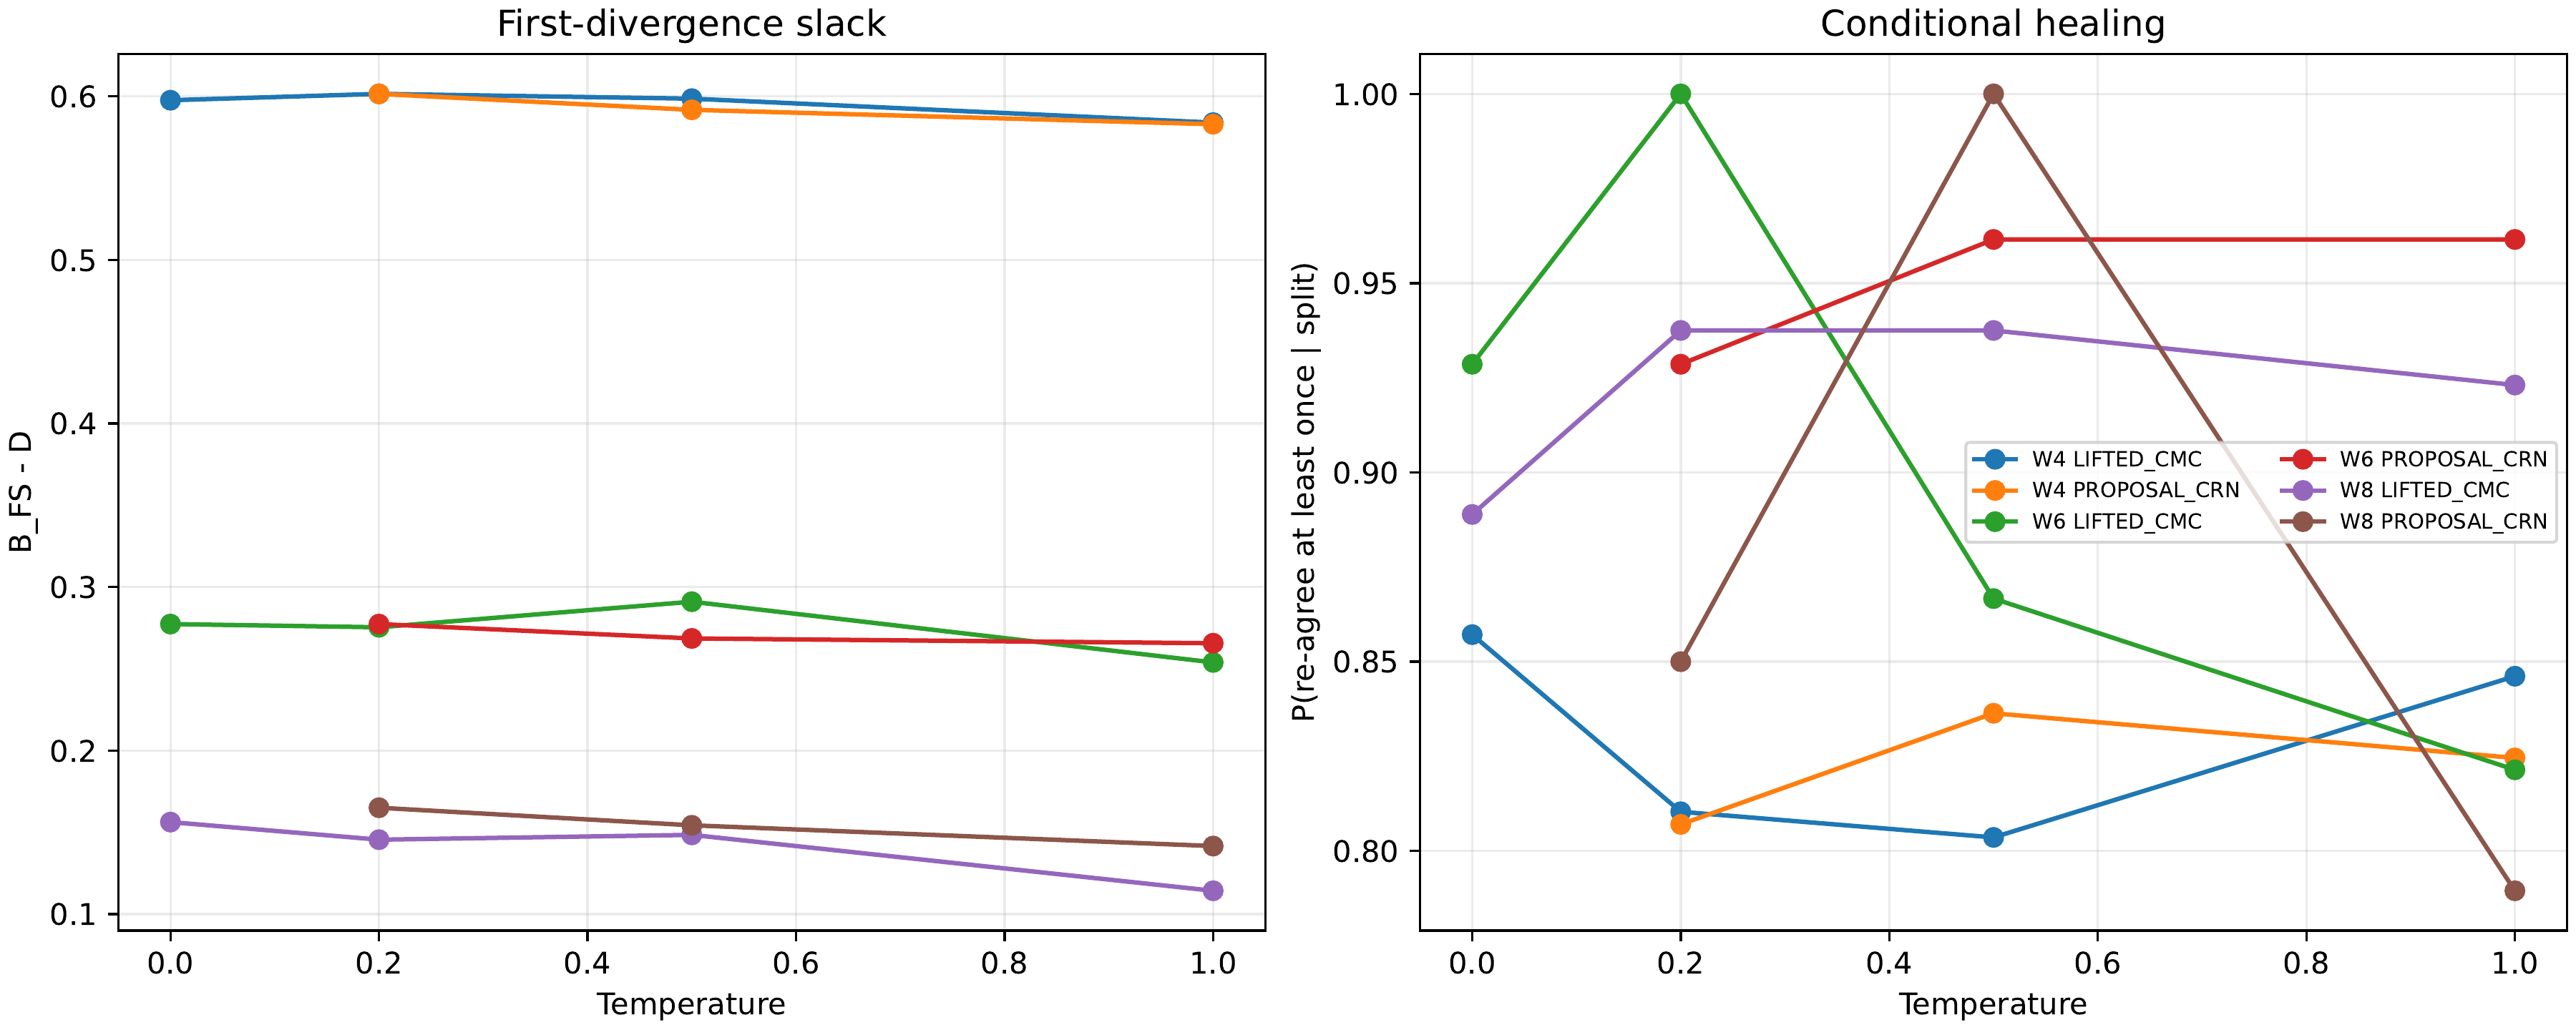
\includegraphics[width=.83\linewidth]{figures/figure_temperature_healing.png}
\caption{First-divergence slack and exact conditional healing. Healing is conditioned on a first split and exhibits the same mixed, bit-dependent ordering as terminal cost.}
\label{fig:app-healing}
\end{figure}

The same-state audit spans early/middle/late states, both precision branches, and 4,000 draws per route. At temperature $1.0$, mean proposal effective support is $1.934$, mean pushed-forward support $1.074$, maximum pushed-forward support $1.449$, and minimum modal probability $0.8173$. Lifted proposal-CMC reduces proposal-vector mismatch from $0.1709$ to $0.0724$, but next-state mismatch remains $0.0146$ versus $0.0142$, demonstrating selector compression.

\subsection{Negative results and interpretation limits}
All relative-to-reference-diversity certificates fail at the preregistered thresholds. First-divergence bounds can be loose because they ignore healing. The temperature comparison is mixed across bit and prompt. Exact-token Hamming is the theorem-aligned metric, not a semantic-quality certificate. The dedicated alternate-metric, lower-bound, and calibration investigations are reported in Appendix~\ref{app:negative}.

\section{Detailed Negative Investigations}
\label{app:negative}

This appendix reports the two preregistered follow-ups summarized in Section~\ref{sec:negative}. Both work packages passed their validity, raw-reconstruction, dual-implementation, and artifact checks. Their scientific gates were negative.

\subsection{General additive token costs}
Let $\Xs=\prod_{i=1}^N\Xs_i$, let each $c_i$ be a metric with $\operatorname{diam}(c_i)\le1$, and define
\[
d_c(x,y)=\sum_{i=1}^N\lambda_i c_i(x_i,y_i),
\qquad \lambda_i>0,\quad \sum_i\lambda_i=1.
\]

\begin{theorem}[Product transport for additive coordinate costs]
\label{thm:general-additive}
If $P=\bigotimes_i p_i$ and $Q=\bigotimes_i q_i$ on finite supports, then
\[
W_{d_c}(P,Q)=\sum_i\lambda_iW_{c_i}(p_i,q_i).
\]
A product of coordinatewise $c_i$-optimal couplings attains the minimum.
\end{theorem}
\begin{proof}
For any coupling $\pi$ of $P$ and $Q$, its coordinate projection $\pi_i$ couples $p_i$ and $q_i$. Hence
\[
\Ex_\pi[d_c(X,Y)]
=\sum_i\lambda_i\Ex_{\pi_i}[c_i(X_i,Y_i)]
\ge\sum_i\lambda_iW_{c_i}(p_i,q_i).
\]
Conversely, finite support gives an optimal coordinate coupling $\pi_i^\star$ for every $i$. Their product couples $P$ and $Q$ and has expected cost equal to the lower bound.
\end{proof}

\begin{corollary}[General-cost first-divergence bound]
\label{cor:general-additive-fs}
For monotone mask-to-token copy-only chains and any valid path coupling $\Gamma$, at a deterministic horizon $r$,
\[
D_\Gamma^{(c)}(r)
\le \Ex_\Gamma\!\left[R_c(X_{\tau^{(r)}})\Ind{\tau^{(r)}\ne\dagger}\right],
\quad
R_c(s)=\sum_{i:s_i=\Mtok}\lambda_i\operatorname{diam}(c_i).
\]
\end{corollary}
\begin{proof}
Before the first split the chains share every committed token. Monotone copy-only evolution preserves those coordinates, so only coordinates still masked in the common pre-split state can differ at the endpoint; coordinate $i$ contributes at most $\lambda_i\operatorname{diam}(c_i)$.
\end{proof}

The empirical study fixes two alternatives without post-hoc tuning. The embedding hybrid is
$0.05\Ind{v\ne w}+0.95\|u_v-u_w\|_2/2$ for frozen normalized input-token embeddings; the byte hybrid replaces the Euclidean term with globally normalized byte-level Levenshtein distance.

\begin{table}[ht]
\caption{W8 CRN saturation. The alternatives change absolute scale but only slightly reduce the ratio to independent-FP variation.}
\label{tab:app-metric-saturation}
\centering\small
\begin{tabular}{@{}lrrr@{}}
\toprule
Metric & FP--W8 CRN & Independent FP & Saturation ratio \\
\midrule
Exact Hamming & 0.91455 & 0.97656 & 0.9365 \\
Embedding hybrid & 0.62349 & 0.67707 & 0.9209 \\
Tokenizer-byte hybrid & 0.06386 & 0.06972 & 0.9159 \\
\bottomrule
\end{tabular}
\end{table}

\begin{figure}[ht]
\centering
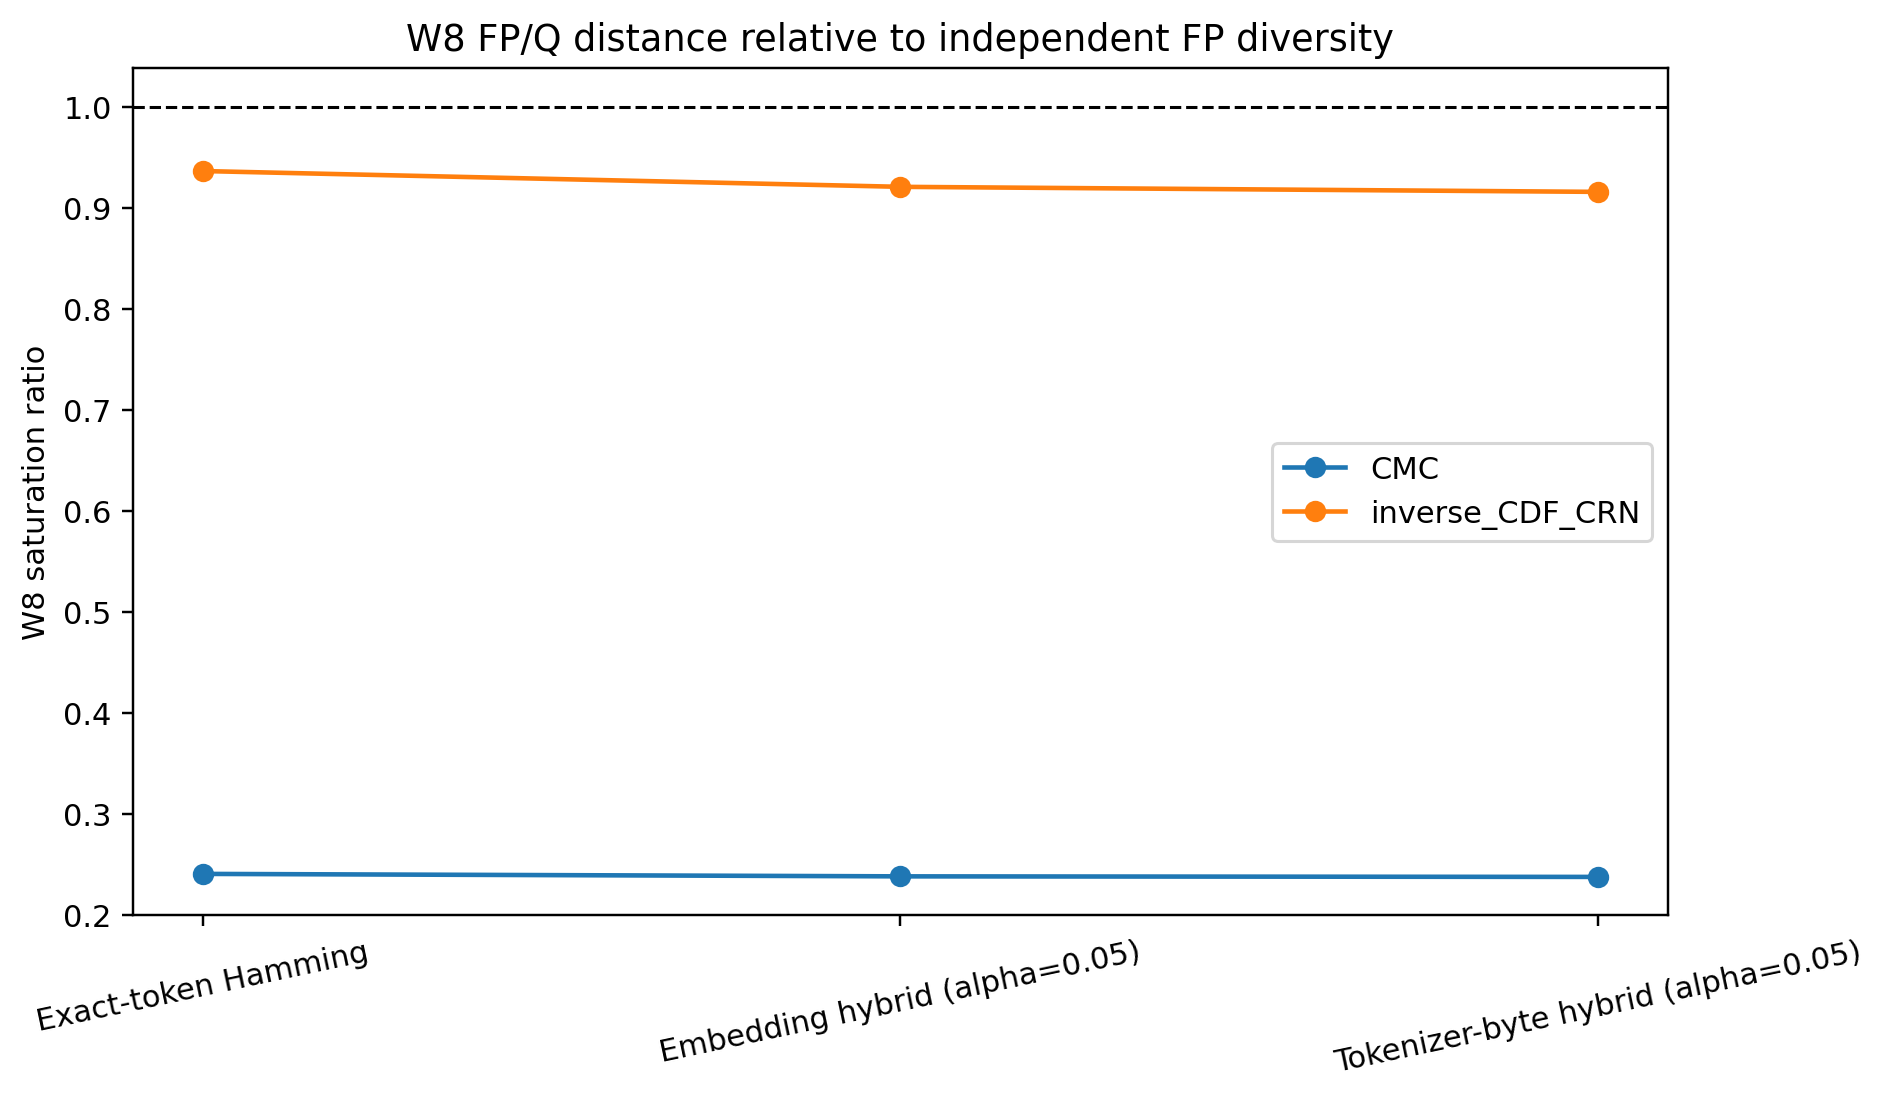
\includegraphics[width=.75\linewidth]{figures/figure_metric_saturation.png}
\caption{Alternative additive token costs do not materially de-saturate the W8 CRN comparison relative to independent-FP variation.}
\label{fig:app-metric-saturation}
\end{figure}

\begin{table}[ht]
\caption{Descriptive GSM8K relevance. The alternative metrics produce almost the same example ordering as Hamming.}
\label{tab:app-metric-task}
\centering\small
\begin{tabular}{@{}lrrr@{}}
\toprule
Metric & Answer-disagreement AUC & Correctness-disagreement AUC & Spearman vs. token edit \\
\midrule
Hamming & 0.9845 & \textbf{0.9573} & 0.99834 \\
Embedding hybrid & 0.9856 & 0.9532 & 0.99845 \\
Tokenizer-byte hybrid & \textbf{0.9876} & 0.9424 & 0.99846 \\
\bottomrule
\end{tabular}
\end{table}

\subsection{Held-out terminal lower-bound witnesses}
Coordinatewise Kantorovich potentials are trained on the fixed 64-prompt suite and frozen before evaluation on 128 disjoint prompt-population draws. The witness is 1-Lipschitz under the corresponding additive metric. A simultaneous empirical-Bernstein lower confidence bound uses the prompt block as the statistical unit.

\begin{table}[ht]
\caption{Held-out witness estimates and formal lower confidence bounds. All simultaneous LCBs are zero. Direct UCBs use the same retained evaluation prompt blocks.}
\label{tab:app-lower-bounds}
\centering\small
\begin{tabular}{@{}clrrr@{}}
\toprule
Bit & Metric & Witness estimate & Formal LCB & Direct CMC UCB \\
\midrule
W8 & Hamming & $-0.00049$ & 0 & 0.4256 \\
W8 & Embedding & $0.00083$ & 0 & 0.3380 \\
W8 & Byte & $-0.00008$ & 0 & 0.1617 \\
W6 & Hamming & $-0.00073$ & 0 & 0.5809 \\
W6 & Embedding & $0.00043$ & 0 & 0.4447 \\
W6 & Byte & $-0.00013$ & 0 & 0.1725 \\
W4 & Hamming & $0.05176$ & 0 & 0.9420 \\
W4 & Embedding & $0.02887$ & 0 & 0.6981 \\
W4 & Byte & $0.00361$ & 0 & 0.1969 \\
\bottomrule
\end{tabular}
\end{table}

\begin{figure}[ht]
\centering
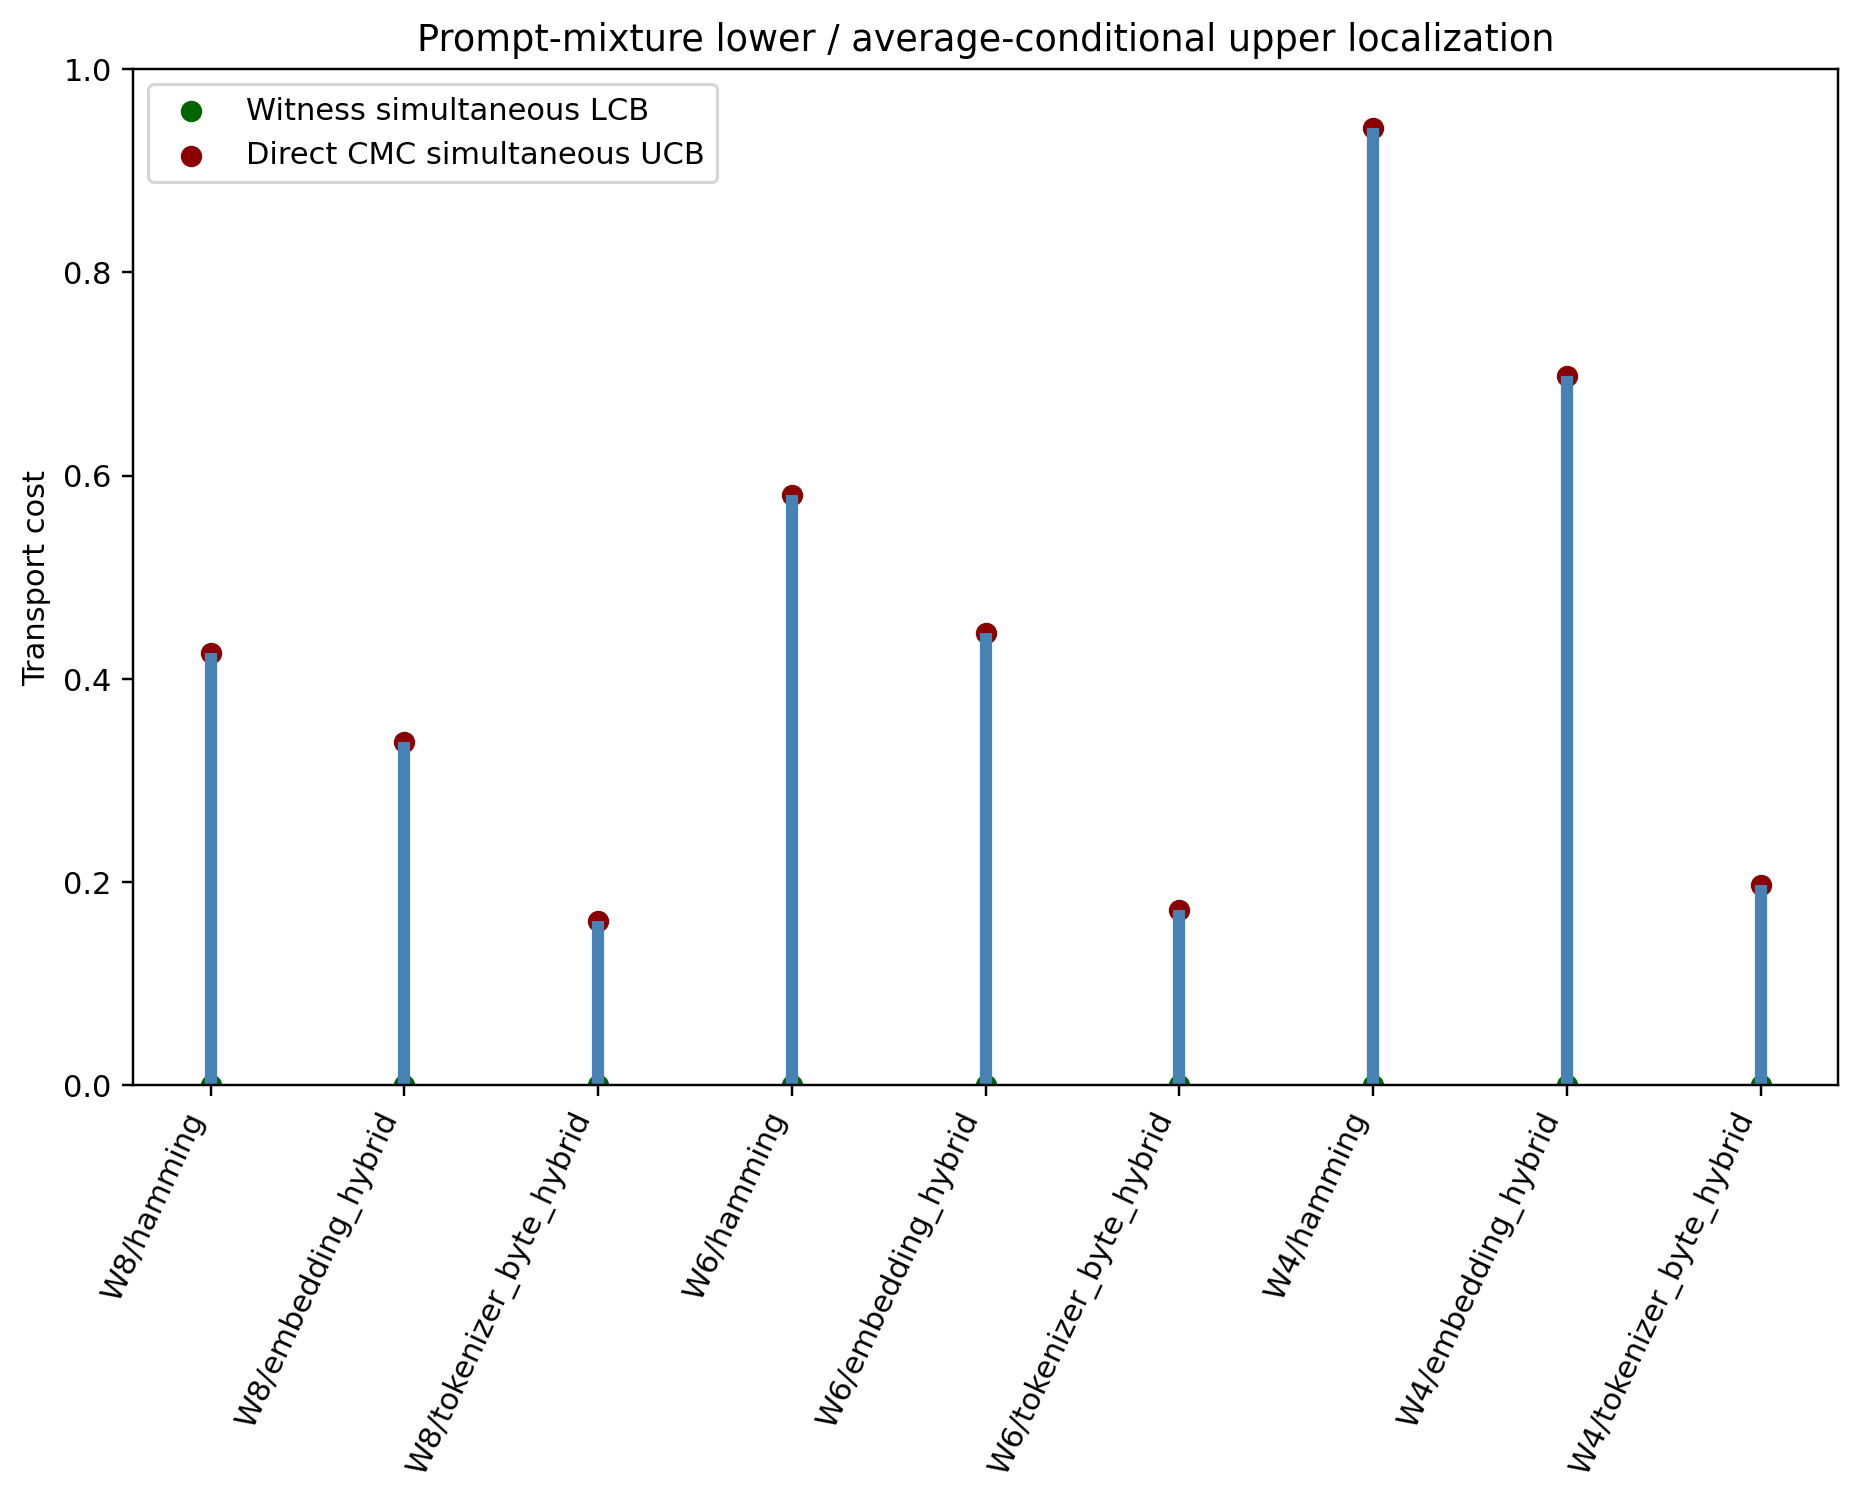
\includegraphics[width=.78\linewidth]{figures/figure_transport_localization.png}
\caption{The held-out point witnesses at W4 are positive, but distribution-free simultaneous lower confidence bounds remain zero. The experiment therefore does not localize terminal Wasserstein distance away from zero.}
\label{fig:app-localization}
\end{figure}

\subsection{Transport-weighted clipping calibration}
The calibration pilot evaluates per-output-row clipping selected with uniform, margin-frontier, residual-only, hazard-only, survival--residual (SR), and survival--residual--hazard (SRH) state weights. The primary W4 endpoint is exact GSM8K accuracy on 512 held-out examples. All methods use the same clipping grid, module set, prompt split, and quantization contract.

\begin{figure}[ht]
\centering
\begin{minipage}[t]{.55\linewidth}
\centering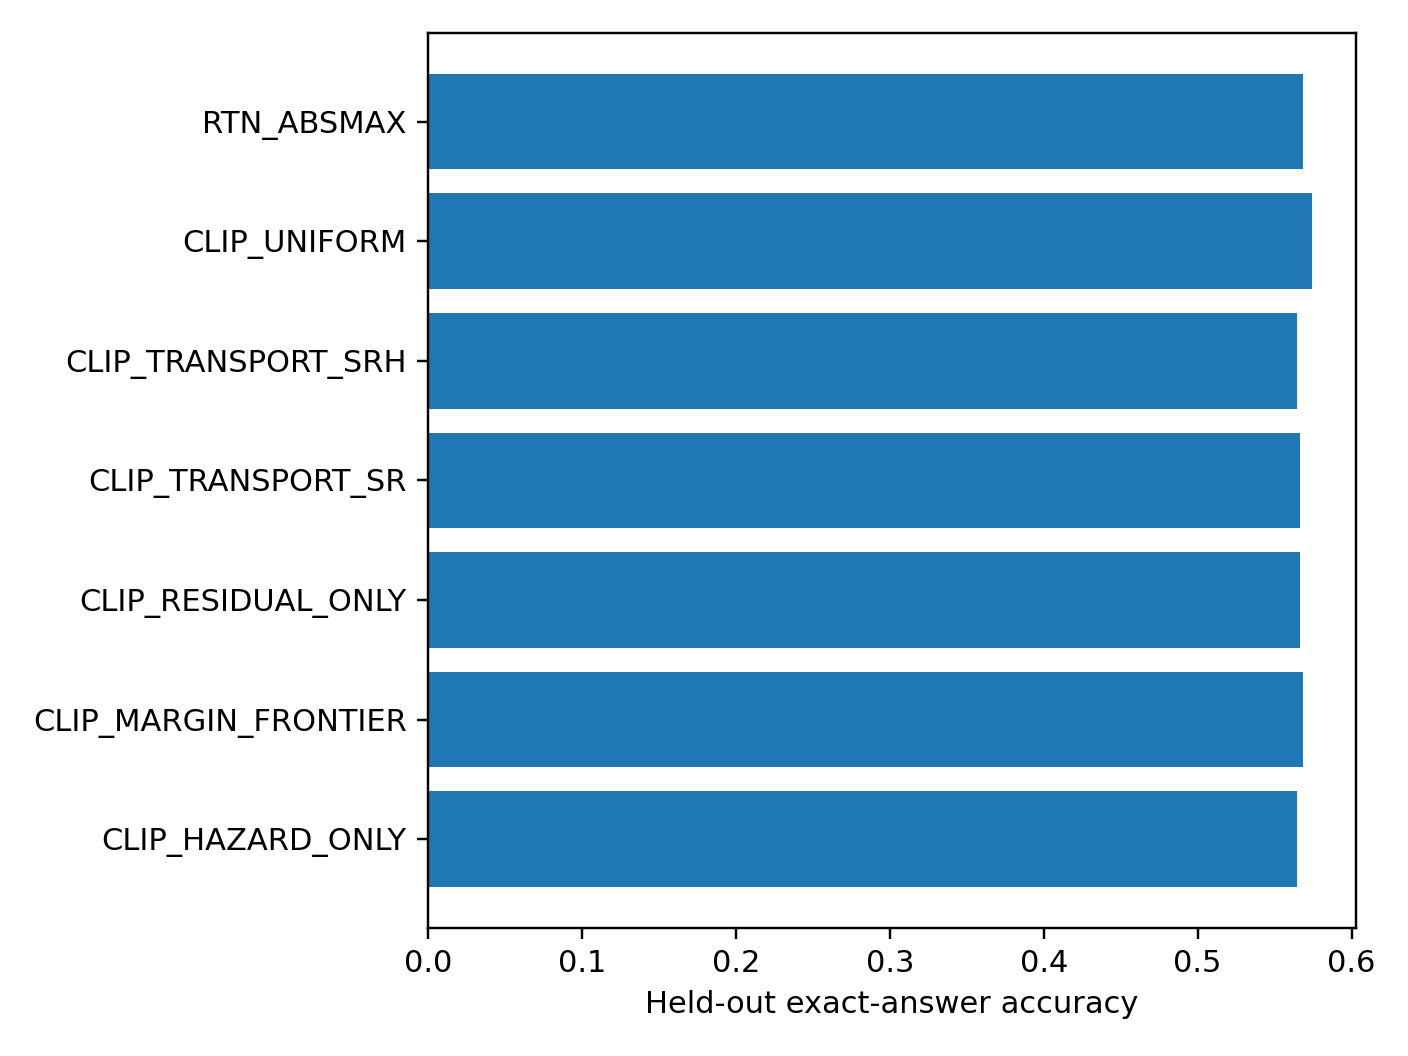
\includegraphics[width=\linewidth]{figures/figure_trcal_w4_accuracy.png}
\end{minipage}\hfill
\begin{minipage}[t]{.42\linewidth}
\centering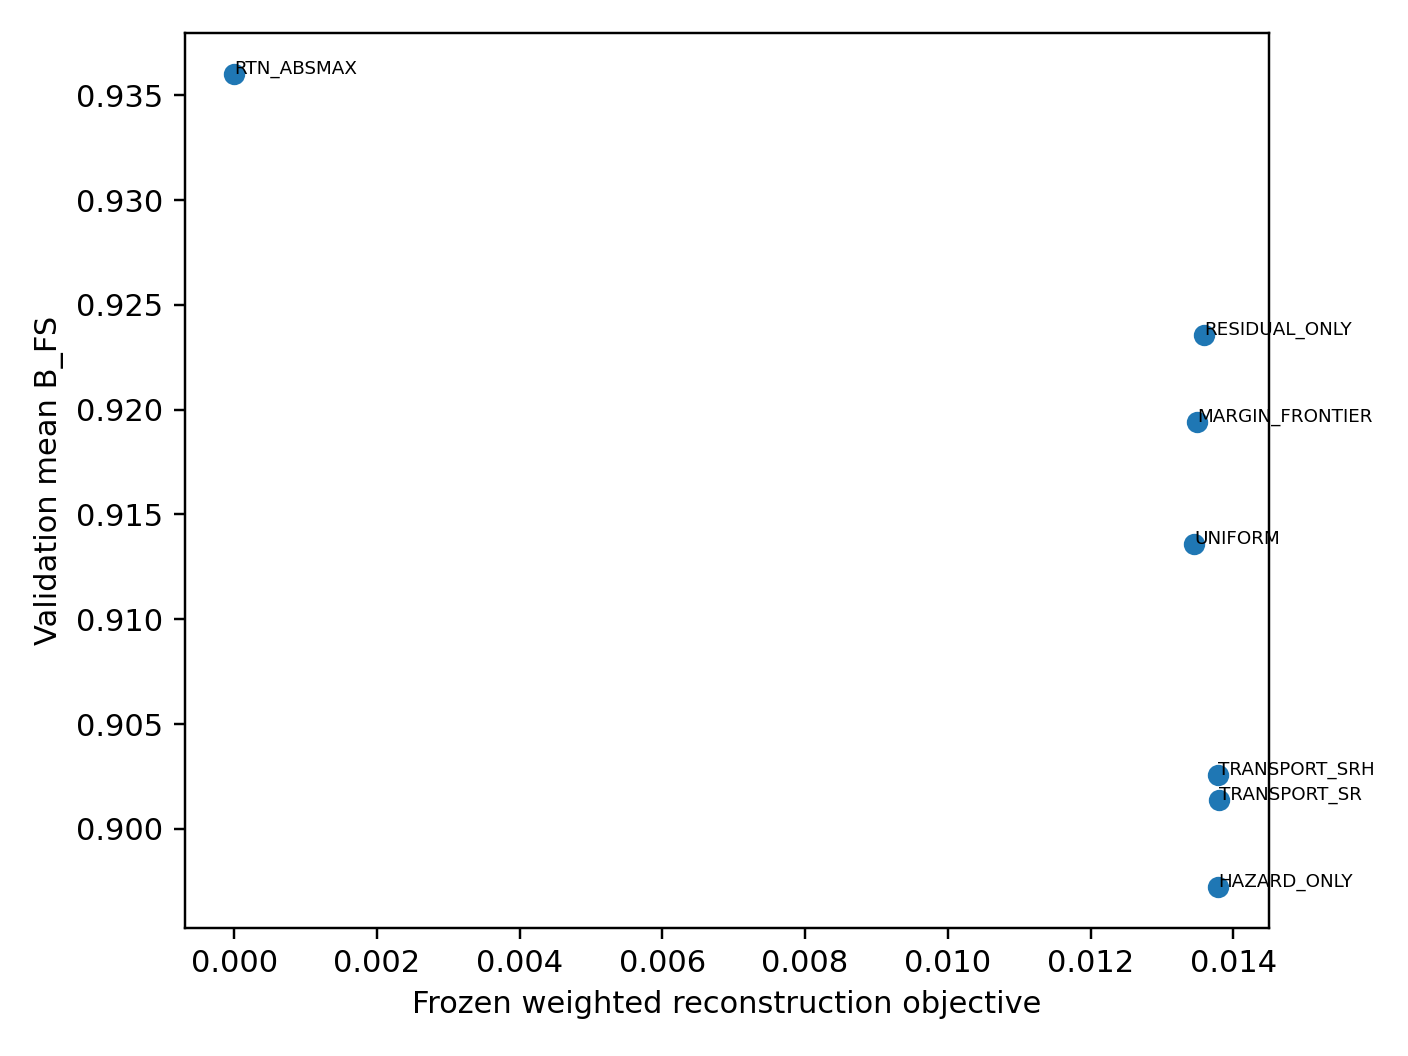
\includegraphics[width=\linewidth]{figures/figure_trcal_bridge.png}
\end{minipage}
\caption{\textbf{Left:} transport-weighted clipping does not improve the primary W4 task endpoint over uniform clipping. \textbf{Right:} the local reconstruction surrogate weakly predicts the next split.}
\label{fig:app-trcal}
\end{figure}

\begin{table}[ht]
\caption{Primary paired W4 comparisons for Transport SR.}
\label{tab:app-trcal-paired}
\centering\small
\begin{tabular}{@{}lrrr@{}}
\toprule
Comparator & Accuracy difference & 95\% paired-bootstrap interval & One-sided McNemar $p$ \\
\midrule
RTN absmax & $-0.20$ pp & $[-1.95,1.37]$ pp & 0.676 \\
Uniform clipping & $-0.78$ pp & $[-1.95,0.39]$ pp & 0.945 \\
Margin frontier & $-0.20$ pp & $[-1.17,0.78]$ pp & 0.773 \\
\bottomrule
\end{tabular}
\end{table}

Transport SR reduces terminal Hamming from $0.0534$ under RTN to $0.0381$ and increases BF16 answer agreement from $84.57\%$ to $89.26\%$, but ground-truth accuracy does not improve. Relative to uniform clipping, it has lower Hamming but lower accuracy and slightly higher $B_{\rm FS}$. The state-level surrogate audit gives split-prediction ROC AUC $0.545$ with interval $[0.479,0.602]$ and Spearman correlation $0.052$ with residual terminal damage. At W3, clipping methods substantially improve over absmax RTN, but SR/SRH are not uniquely better than uniform or margin-frontier calibration.

\subsection{Interpretation}
The negative findings rule out specific stronger stories, not the primary framework. The tested static token costs are not semantic metrics; the frozen prompt-independent witness does not yield a positive population LCB; and the tested local reconstruction objective does not reliably proxy first-split risk. Accordingly, no claim is made that the framework identifies the true terminal Wasserstein distance, supplies a task-improving quantizer, or certifies semantic quality.

\section{Reproducibility and Artifact Map}
\label{app:repro}

\subsection{Release structure}
The public source package contains the complete manuscript, TMLR style file, every displayed figure, and plotted-data CSVs for newly generated summary figures. The experimental artifact is organized into immutable work packages. Each package records configuration, model/checkpoint and tokenizer identities, prompt manifests, event-addressed RNG contracts, row-level results, tests, reports, and SHA-256 manifests. Public checkpoints and datasets are referenced by immutable identifiers rather than duplicated.

\begin{table}[ht]
\caption{Source-to-claim map for the primary and negative work packages.}
\label{tab:artifact-map}
\centering\small
\begin{tabular}{@{}p{.22\linewidth}p{.30\linewidth}p{.38\linewidth}@{}}
\toprule
Package family & Main paper role & Reproduction target \\
\midrule
WP05A/WP05B & local mismatch and split consequence & flip rates, early/middle/late damage \\
CERT-3/CERT-3R & fixed-suite coupling and certificate & CRN/CMC costs, UCBs, horizons, pathwise audit \\
WP07C & declared prompt population & source contract, block UCBs, horizons \\
WP07B & finite-bit scaling & W3--W8 slopes and stress point \\
WP07D & second model and task panel & SMDM length transfer, GSM8K relevance \\
LOCAL-LIFT/TEMP & official selector and temperature & proposal lifting, stochastic stress, healing \\
METRIC-LOC-1 & negative metric/lower-bound study & additive costs, witnesses, zero formal LCBs \\
TRCAL-1 & negative calibration study & state weights, clipping scales, held-out task comparison \\
\bottomrule
\end{tabular}
\end{table}

\subsection{Model-free reproduction}
Each work package provides a model-free command that reconstructs its derived tables, simultaneous bounds, horizon decisions, figure data, and gates from frozen raw outputs. Independent secondary implementations recalculate the load-bearing arithmetic without importing the primary aggregation helpers. The healing correction reconstructs split and re-agreement counts from checkpoint JSON rather than report prose. The metric and calibration investigations similarly preserve their preregistered negative gates.

\subsection{Randomness and pathwise auditing}
Random events are addressed by semantic keys including prompt, bit, draw, reverse step, branch, position, and subevent. Reordering branches or positions therefore does not change the generated random event. This contract was introduced after a stateful-RNG implementation produced 809 apparent pathwise violations that disappeared under event-addressed replay. Every final release checks duplicate event keys, replay, branch and iteration order, fixed commit counts, copy-only state monotonicity, and $D_H\le B_{\rm FS,H}$ at every recorded horizon.

The five initial pathwise families contribute
$8{,}064+6{,}048+6{,}048+3{,}072+1{,}632=24{,}864$ checks. The official-sampler temperature extension contributes $4{,}800$, for $29{,}664$ recorded checks total, all with zero violation. These counts are dependent audit totals; they are not used as confidence-sample sizes.

\subsection{Statistical units}
Fixed-suite statements average over frozen prompts and the declared independently addressed coupling draws. The conservative sensitivity first averages draws within each prompt. Prompt-population statements first average repeated draws within each IID prompt block and apply concentration across prompt blocks. Bootstrap analyses resample the top-level prompt or example block. Tokens, reverse steps, horizons, and multiple methods on one example are never treated as independent statistical observations.

\subsection{Anonymity and release hygiene}
The public preprint package removes usernames, local absolute paths, credentials, private repository URLs, and personal storage links. The public PDF and metadata identify Munsik Kim as the author. Any future double-blind venue submission must use a separately generated anonymous manuscript and supplementary package, must not link to this archive during review unless the venue policy explicitly permits it, and must preserve the same scientific source hashes and manifests.

\subsection{Claim boundaries encoded in the artifacts}
Gates distinguish validity from scientific outcome. For example, the metric-localization and transport-calibration packages pass implementation and reproducibility checks but retain negative scientific labels. Reports explicitly prohibit interpreting token embeddings as semantic metrics, plug-in OT as a certified population lower bound, proposal maximality as terminal optimality, or BF16 fidelity as task improvement. This prevents later artifact users from converting failed preregistered hypotheses into unsupported positive claims.


\end{document}
